\PassOptionsToPackage{numbers,compress}{natbib}
\documentclass{article}

% arXiv / preprint version
\usepackage[preprint]{neurips_2025}

\usepackage[utf8]{inputenc}
\usepackage[T1]{fontenc}
\usepackage{hyperref}
\usepackage{url}
\usepackage{booktabs}
\usepackage{amsfonts}
\usepackage{amsmath,amssymb,mathtools}
\usepackage{nicefrac}
\usepackage[table]{xcolor}

% ---------- table colors ----------
\definecolor{TabHeader}{HTML}{D9E4F2}   % 顶部表头：冷灰蓝
\definecolor{TabGroup}{HTML}{EEF2F7}    % 分组条：浅灰蓝
\definecolor{TabOffline}{HTML}{F4EEF9}  % Batch,S3：淡紫
\definecolor{TabSingle}{HTML}{EAF4FF}   % single-turn,S3：淡蓝
\definecolor{TabMulti}{HTML}{EAF8F1}    % multi-turn,S3：淡绿

\arrayrulecolor{black}

\usepackage{graphicx}
\usepackage{multirow}
\usepackage{float}
\usepackage{capt-of}
\usepackage{fvextra}
\usepackage{enumitem}
\usepackage[capitalize,noabbrev]{cleveref}

\DefineVerbatimEnvironment{PromptBox}{Verbatim}{
  fontsize=\footnotesize,
  breaklines=true,
  breakanywhere=true,
  frame=single,
  framesep=2mm
}

% Small layout tuning for the NeurIPS template
\setlist[itemize]{leftmargin=1.3em,itemsep=2pt,topsep=3pt,parsep=0pt,partopsep=0pt}
\setlist[enumerate]{leftmargin=1.5em,itemsep=2pt,topsep=3pt,parsep=0pt,partopsep=0pt}
\setlength{\textfloatsep}{10pt plus 2pt minus 2pt}
\setlength{\floatsep}{8pt plus 2pt minus 2pt}
\setlength{\intextsep}{8pt plus 2pt minus 2pt}
\setlength{\abovecaptionskip}{4pt}
\setlength{\belowcaptionskip}{2pt}

% Table colors
\definecolor{TableHeader}{RGB}{244,247,252}
\definecolor{TableSection}{RGB}{232,239,251}
\definecolor{TableHighlight}{RGB}{240,245,255}

\title{Think While Watching: Online Streaming Segment-Level Memory for Multi-Turn Video Reasoning in Multimodal Large Language Models}

\author{
Lu Wang$^{1}$ \quad
Zhuoran Jin$^{1}$ \quad
Yupu Hao$^{1}$ \quad
Yubo Chen$^{1}$ \\
Kang Liu$^{1}$ \quad
Yulong Ao$^{2}$ \quad
Jun Zhao$^{1}$ \\
$^{1}$The Key Laboratory of Cognition and Decision Intelligence for Complex Systems,\\
Institute of Automation, Chinese Academy of Sciences, Beijing, China \\
$^{2}$Beijing Academy of Artificial Intelligence (BAAI), Beijing, China \\
\texttt{wanglu2026@ia.ac.cn, zhuoran.jin@nlpr.ia.ac.cn, haoyupu2023@ia.ac.cn} \\
\texttt{yubo.chen@nlpr.ia.ac.cn, kliu@nlpr.ia.ac.cn} \\
\texttt{aoyulong@outlook.com, jzhao@nlpr.ia.ac.cn}
}

\begin{document}

\maketitle

\begin{abstract}
Multimodal large language models (MLLMs) have demonstrated strong performance in offline video understanding tasks, but most remain constrained to offline inference or exhibit weak online reasoning ability, rendering online multi-turn interaction over continuously arriving video streams challenging. Existing streaming approaches adopt an interleaved perception-generation paradigm, which precludes concurrent perception and generation and induces early memory decay with growing streams, degrading long-range dependency modeling. We propose \textbf{Think While Watching}, a memory-anchored streaming video reasoning framework that maintains continuous segment-level memory during multi-turn interaction. We construct a three-stage, multi-round, chain-of-thought (CoT) dataset with a stage-matched training strategy while enforcing strict causality in streaming reasoning via a segment-level streaming causal mask and streaming positional encoding. At inference, we design an efficient pipeline that overlaps watching and thinking and adaptively selects the optimal attention backend. We evaluate our method under single-round and multi-round streaming input protocols. Based on Qwen3-VL, we improve single-round accuracy by 2.6\% on StreamingBench and 3.79\% on OVO-Bench. In the multi-round protocol, we maintain performance while reducing output tokens by 56\%. Our code is available at \href{https://github.com/wl666hhh/Think_While_Watching/}{GitHub}.
\end{abstract}

\section{Introduction}

\begin{figure*}[t]
  \centering
  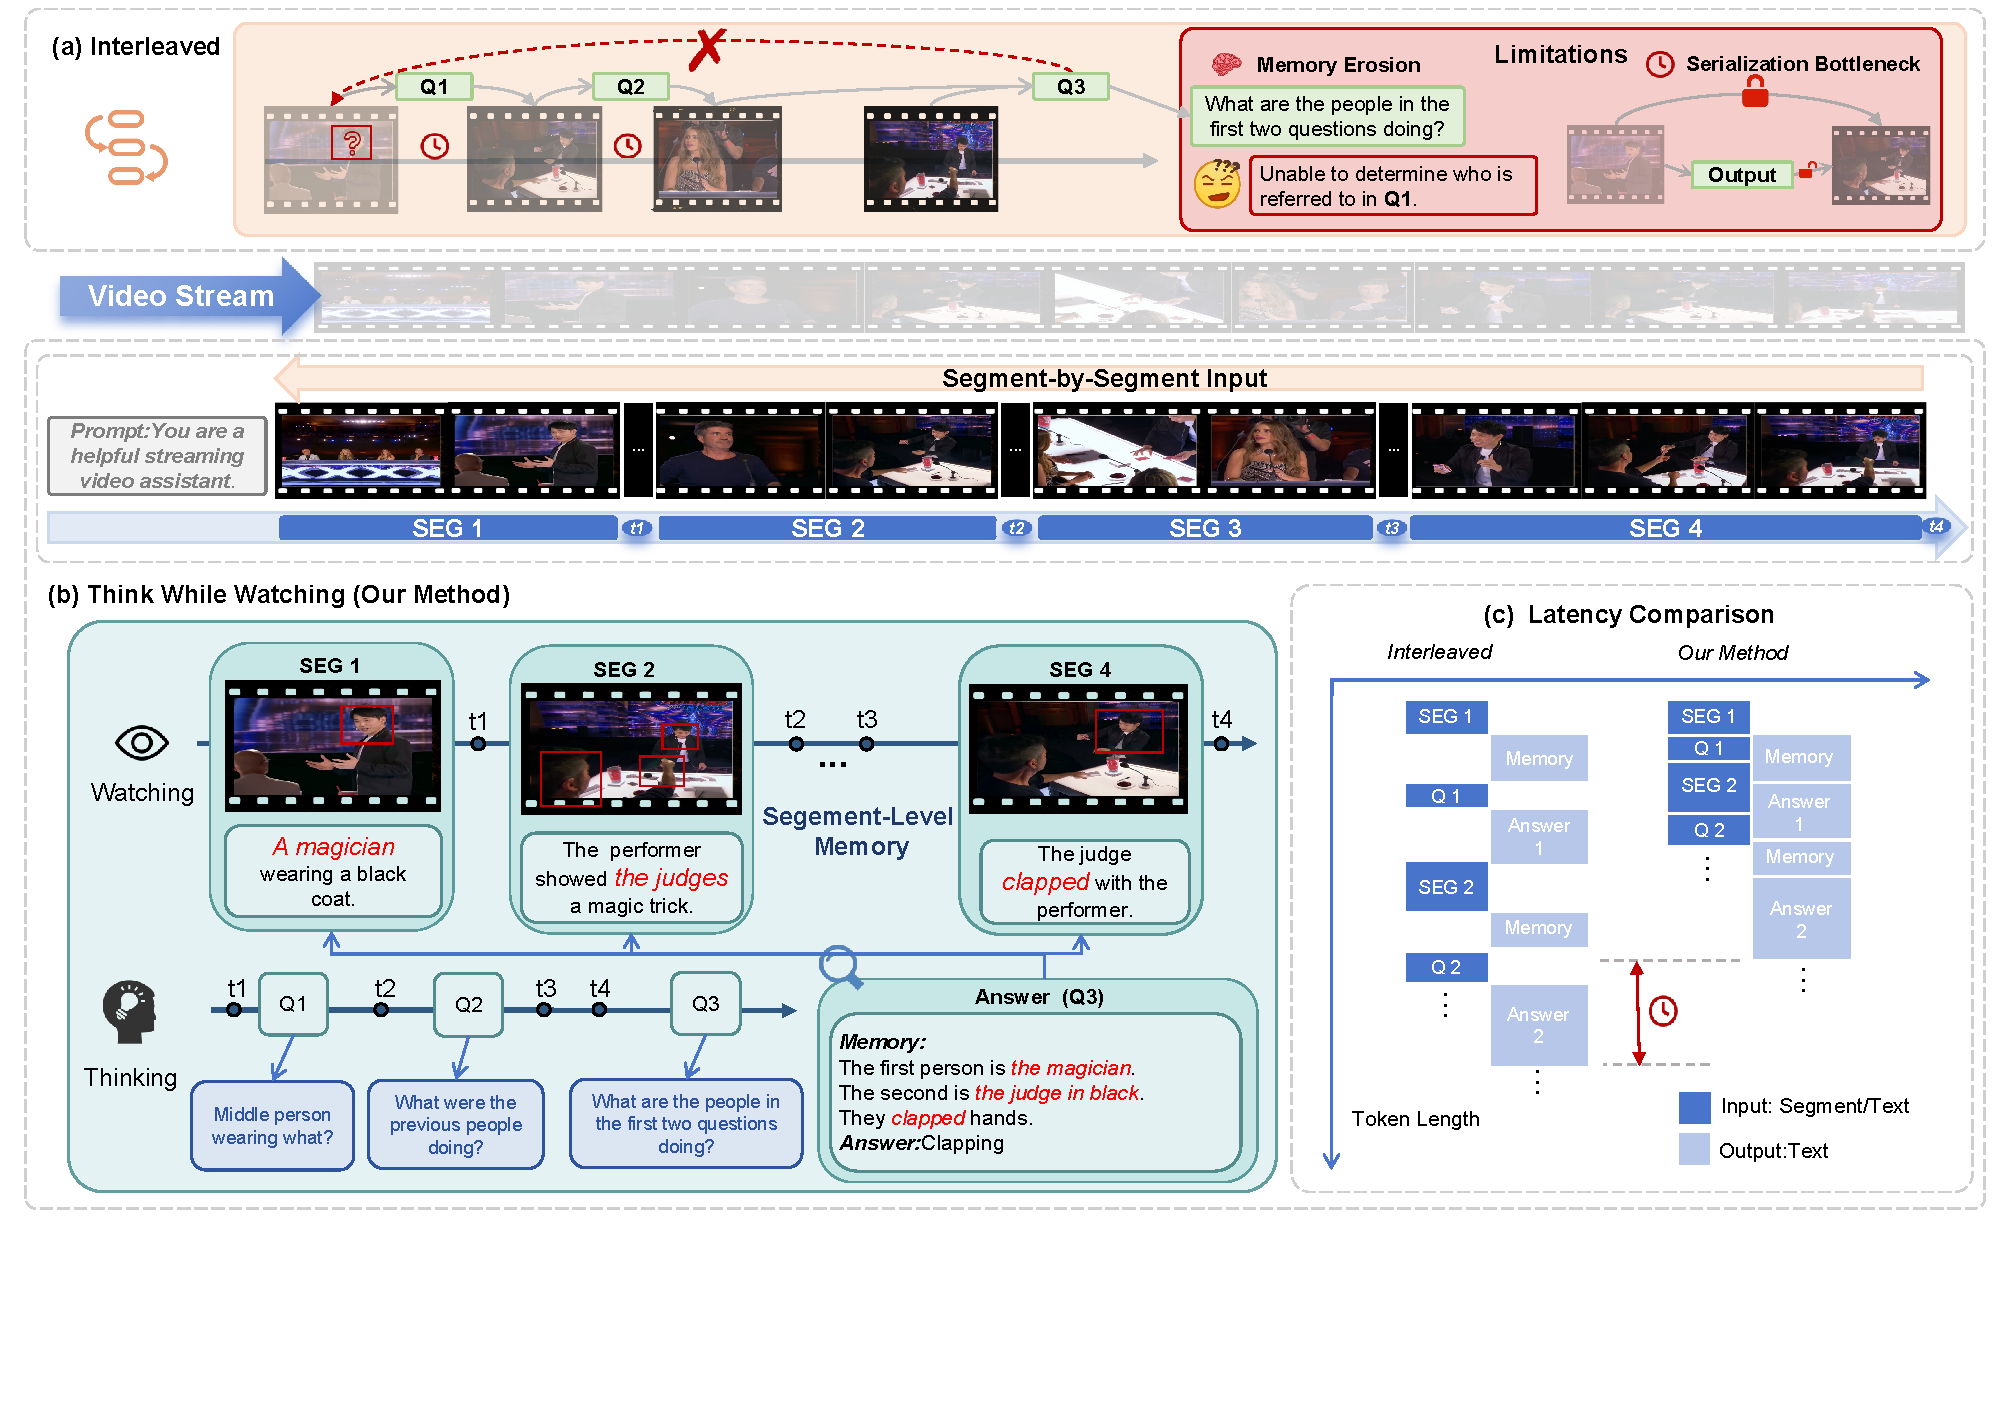
\includegraphics[width=\linewidth]{Figure/F1.pdf}
  \caption{\textbf{Overview of Think While Watching.}
  \textbf{(a) Interleaved baseline.} Video perception and answer generation are executed sequentially, which can cause \textbf{memory erosion}, where early memory is forgotten, and a \textbf{serialization bottleneck}, where generation stalls further input ingestion.
  \textbf{(b) Think While Watching (ours).} The video frames are processed in segments (SEG 1 to SEG 4) to build a continuous \textbf{segment-level memory}. During streaming, questions are answered online by retrieving implicitly relevant memories while continuing to watch.
  \textbf{(c) Latency comparison.} A schematic timeline showing that interleaved processing accumulates queueing delay, while our decoupled design parallelizes segment processing and answering to reduce latency.}
  \label{fig:main}
\end{figure*}

Video understanding and reasoning are becoming central capabilities for multimodal assistants. While multimodal large language models (MLLMs) have achieved strong performance in offline video benchmarks where the full video is available before inference in a single-turn setting \cite{DBLP:journals/corr/abs-2511-04570,DBLP:journals/corr/abs-2508-04416,DBLP:journals/corr/abs-2503-21776,DBLP:journals/corr/abs-2501-03230}, many high-impact scenarios are inherently \textbf{streaming}: live broadcasting \cite{DBLP:journals/corr/abs-2511-05299,DBLP:conf/cvpr/ChenZLLMS25}, monitoring, robotic assistants \cite{wang2025streameqastreamingvideounderstanding}, and other streaming scenarios. In these settings, users may ask questions at any time, and the assistant must answer in real time while staying faithful to the visual evidence observed so far, especially under \textbf{multi-turn} interaction, where later questions often depend on earlier memories.

A widely adopted approach for streaming MLLMs is to interleave perception and generation \cite{DBLP:conf/cvpr/ChenLWLSGLGMS24,DBLP:journals/corr/abs-2412-08646,DBLP:conf/cvpr/ChenZLLMS25}. Although this reduces delay compared to offline approaches, it remains fundamentally serialized: text decoding blocks further video ingestion. This interleaved pattern leads to two phenomena.
First, \textbf{Memory Erosion}: multi-turn subsequent questions frequently refer back to earlier questions or earlier visual cues, but interleaving with generation tends to erode long-range capability. The failure case in Fig.~\ref{fig:main}(a) makes this explicit: a later query about the first two questions becomes unanswerable because the model forgets who Q1 refers to. This issue is also validated by our experimental results: for the Qwen3-VL-4B Thinking model, accuracy in the online multi-round setting drops $40.39\%$ compared to the offline setting, highlighting the severe challenge of maintaining long-term temporal consistency.
Second, \textbf{Serialization Bottleneck}: as illustrated on the top right of Fig.~\ref{fig:main}(a), once the model starts generation, the decoder effectively locks the streaming sequence, directly harming responsiveness in dynamic streams. The root cause is that autoregressive models use unified positional encoding, so new inputs must align with generated outputs whose length is unknown, forcing ingestion to pause and causing a serialization bottleneck. Fig.~\ref{fig:main}(c) further visualizes this effect: under interleaved processing, as the number of rounds accumulates, the input keeps piling up, leading to increasing end-to-end latency. To mitigate \textbf{Memory Erosion}, we make memory writing an explicit online behavior: for each observed segment, the model writes a memory note and appends it to a memory bank; when a question arrives, the model answers by implicitly integrating the relevant notes via the attention mechanism in Fig.~\ref{fig:main}(b). To break the \textbf{Serialization Bottleneck}, we assign independent positional encodings to decouple input and output streams at inference time, enabling input-output parallelism so the model can keep watching while thinking and thus reduce latency.

We propose \textbf{Think While Watching}, a memory-anchored streaming video reasoning framework for online multi-turn interaction. We represent a continuously arriving video as a sequence of segments and maintain a persistent \textbf{segment-level memory} throughout the dialogue. To make the framework practical, we design corresponding training and inference procedures. On the training side, we construct a three-stage, multi-round chain-of-thought (CoT) dataset with training matched to each stage, together with a \textbf{segment-level streaming causal mask} and \textbf{streaming positional encoding}, which jointly enforce strict causality throughout streaming reasoning. On the inference side, we design an efficient pipeline that overlaps watching with thinking. Our implementation is inspired by CPU process scheduling \cite{DBLP:books/wi/SGG2018} in operating systems: we organize inference as a \textbf{multi-stage pipeline} as illustrated in Fig.~\ref{fig:main}(c) and decouple continuous visual ingestion from text decoding via a dual KV cache \cite{DBLP:conf/acl/TongFLFZSS25,DBLP:journals/corr/abs-2510-17238,lin2026speakwatchingunleashingtrue}, enabling parallelism between perception and generation and mitigating serialization.

We evaluate Think While Watching under two streaming input protocols: \textbf{single-round}, where the input contains many arriving segments but the assistant answers one question, and \textbf{multi-round}, where the input contains many arriving segments and the assistant answers multiple questions over time. In the Qwen3-VL family, we improve single-round accuracy by 2.6\% on StreamingBench and 3.79\% on OVO-Bench. In the multi-round protocol, we preserve performance while reducing output tokens by 56\%.

\noindent\textbf{Our contributions} are as follows:
\begin{itemize}
  \item We propose \textbf{Think While Watching}, which maintains \textbf{segment-level memory} as a persistent state and answers each query by implicitly retrieving and integrating relevant memories, improving multi-turn consistency and enabling decoupled perception and generation. We further provide a practical \textbf{training and inference} pipeline with \textbf{three-stage training}, \textbf{streaming segment masking}, and \textbf{streaming positional encoding} for causal segment-level modeling, and a dual KV cache at inference time to support parallelism between perception and generation.
  \item We construct a three-stage, stage-aligned streaming CoT dataset with multi-round dialogues to support the proposed training strategy.
  \item On Qwen3-VL, we improve single-round accuracy by 2.6\% on StreamingBench and 3.79\% on OVO-Bench, while in multi-round streaming, we reduce output tokens by 56\% without accuracy drop.
\end{itemize}

\section{Related Work}

\subsection{Offline Video Understanding}
Offline video MLLMs are improved by structured perception and cognition pipelines and temporal reasoning designs \cite{DBLP:journals/corr/abs-2501-03230,DBLP:journals/corr/abs-2511-04570,DBLP:journals/corr/abs-2508-04416}, and by reinforcement learning for complex temporal reasoning \cite{DBLP:journals/corr/abs-2503-21776,DBLP:journals/corr/abs-2507-07966}. Most of these methods assume the full video is available before answering, leaving causal online multi-turn interaction less explored.

\subsection{Online Streaming Video Understanding}

\noindent\textbf{Benchmarks.}
StreamingBench evaluates the gap between offline models and streaming video understanding \cite{lin2024streamingbenchassessinggapmllms}, while OVO-Bench emphasizes real-world online video understanding \cite{DBLP:conf/cvpr/NiuLMGZHDDD0ZZC25}. Recent work further studies streaming along with active perception and multi-turn interaction \cite{Yang2025ViSPeak,lee2025streamgazegazeguidedtemporalreasoning,DBLP:journals/corr/abs-2510-14560,DBLP:conf/iclr/YangHDXQW0DX25,DBLP:journals/corr/abs-2505-02064}.

\noindent\textbf{Interleaved perception and generation.}
Many streaming systems alternate visual ingestion and text decoding, as in VideoLLM-online \cite{DBLP:conf/cvpr/ChenLWLSGLGMS24} and StreamChat \cite{DBLP:journals/corr/abs-2412-08646}, and scale streaming supervision for online interaction \cite{DBLP:conf/cvpr/ChenZLLMS25,DBLP:journals/corr/abs-2510-09608}. This coupling limits input-output parallelism and makes it harder to model dependencies over a long horizon across multiple turns.

\noindent\textbf{Memory and efficient inference for long-horizon streaming.}
For efficiency, one line reduces redundant visual tokens in streaming videos \cite{DBLP:journals/corr/abs-2504-17343,DBLP:conf/cvpr/ZhouABYMXNS24,DBLP:journals/corr/abs-2510-18269,DBLP:conf/iclr/XiongYYZ0ZL25}. Another line reuses historical context via KV cache retrieval and compression \cite{kim2025vrexrealtimestreamingvideo,DBLP:journals/corr/abs-2511-07278,DBLP:conf/iclr/DiYZLZCLHSJ25,DBLP:journals/corr/abs-2505-15269,DBLP:journals/corr/abs-2505-13140,DBLP:journals/corr/abs-2506-23825}. Persistent memory and long-term multimodal agent memory further support evidence reuse across long streams \cite{DBLP:journals/corr/abs-2509-24871,DBLP:journals/corr/abs-2508-09736,DBLP:journals/corr/abs-2508-01875}. Our work emphasizes stable segment-level memory for multi-turn streaming and an inference design that keeps perception and generation decoupled.

\section{Preliminary}
\label{sec:paradigm}

This section introduces the online multi-turn streaming video question answering setting studied in this work. A video is observed sequentially as a stream of segments, while a user may ask questions at arbitrary segment boundaries. The central requirement is strict streaming causality: at each turn, the system must produce its response using only the video content observed so far and the dialogue history, without accessing any future segments.

\subsection{Streams and Turns}
\label{sec:paradigm:stream}

\noindent\textbf{Segmented stream.}
We represent a video stream as an ordered sequence of segments
\begin{equation}
\mathbf{S}_{1:T} \triangleq \langle \mathbf{S}_1,\ldots,\mathbf{S}_T\rangle ,
\end{equation}
where each $\mathbf{S}_t$ denotes a contiguous chunk of frames. Segments arrive in temporal order, and the system processes them online.

\noindent\textbf{Multi-turn questioning.}
We consider an interaction with $R$ question and answer turns. At turn $r \in \{1,\ldots,R\}$, the user asks a question $q_r$ after the system has observed a prefix of the stream. Let $\tau_r \in \{1,\ldots,T\}$ denote the index of the latest observed segment when $q_r$ is issued. Equivalently, $q_r$ is asked after ingesting the segment prefix
\begin{equation}
\mathbf{S}_{1:\tau_r} \triangleq \langle \mathbf{S}_1,\ldots,\mathbf{S}_{\tau_r}\rangle .
\end{equation}
Since questions arrive over time, the indices are nondecreasing:
\begin{equation}
1 \le \tau_1 \le \tau_2 \le \cdots \le \tau_R \le T .
\end{equation}
The dialogue history before turn $r$ is
\begin{equation}
\mathcal{H}_{r-1} \triangleq \langle \langle q_1,a_1\rangle,\ldots,\langle q_{r-1},a_{r-1}\rangle\rangle .
\end{equation}
Under strict causality, the answer $a_r$ at turn $r$ is conditioned only on the observed video prefix $\mathbf{S}_{1:\tau_r}$, the question $q_r$, and the dialogue history $\mathcal{H}_{r-1}$.

\subsection{Streaming Protocols}
\label{sec:paradigm:protocols}

We consider two online evaluation protocols that share the same segmented stream $\mathbf{S}_{1:T}$ but differ in the number of question turns.

\noindent\textbf{Single-round streaming.}
Only one question is asked, so $R=1$. The system processes segments online and produces a single output for the question asked at $\tau_1$. We denote the model output as $\langle \pi_1, a_1\rangle$, where $\pi_1$ is an optional intermediate rationale such as chain of thought and $a_1$ is the final answer.

\noindent\textbf{Multi-round streaming.}
Multiple questions are asked, so $R>1$, at different times with nondecreasing $\tau_r$. At each turn $r$, the system must answer online using only the stream prefix $\mathbf{S}_{1:\tau_r}$ and the dialogue history $\mathcal{H}_{r-1}$, producing an output pair $\langle \pi_r, a_r\rangle$.

\subsection{Streaming Unit Notation}
\label{sec:paradigm:notation}

To describe training and inference in a single causal formulation, we serialize a streaming interaction as an interleaved sequence of received units and a one-to-one aligned sequence of generated units.

\noindent\textbf{Received units.}
Let the received unit sequence be
\begin{equation}
\mathbf{R}_{1:U} \triangleq \langle R_1,\ldots,R_U\rangle ,
\end{equation}
where each $R_u$ is either a visual segment unit $S_t$ that contains the content of $\mathbf{S}_t$, or a question unit $Q_r$ that contains the text $q_r$. We write $R_u \in \{S,Q\}$ to indicate the unit type. Let $\operatorname{idx}\lbrack \cdot \rbrack$ return the arrival index in $\mathbf{R}_{1:U}$, so $\operatorname{idx}\lbrack S_t \rbrack$ is the index $u$ where segment $t$ appears, and $\operatorname{idx}\lbrack Q_r \rbrack$ is the index $u$ where question $r$ appears.

\noindent\textbf{Generated units.}
For each received unit $R_u$, the model generates exactly one output unit $C_u$ in the same order, forming
\begin{equation}
\mathbf{C}_{1:U} \triangleq \langle C_1,\ldots,C_U\rangle .
\end{equation}
If $R_u=S_t$, then $C_u$ is a memory note denoted $m_t$. If $R_u=Q_r$, then $C_u$ is the question answering output that contains the rationale $\pi_r$ and answer $a_r$.

\noindent\textbf{Token lengths and visual grids.}
For any text unit $Y$ in $\{Q_1,\ldots,Q_R,C_1,\ldots,C_U\}$, let $L\lbrack Y \rbrack$ denote its text token length. For any segment unit $S_t$, let its visual token grid sizes be $\langle T_t,H_t,W_t\rangle$. Here $T_t$ is the number of visual tokens along the temporal axis, $H_t$ is the height axis, and $W_t$ is the width axis, defined by the vision encoder token grid for this segment. We will also use a unit span function $\Delta\lbrack R_u \rbrack$ that assigns each received unit a nonoverlapping input position span:
\begin{equation}
\Delta\lbrack R_u \rbrack =
\begin{cases}
\max\{T_u,H_u,W_u\}, & R_u \in \{S\},\\
L\lbrack R_u \rbrack, & R_u \in \{Q\}.
\end{cases}
\label{eq:delta}
\end{equation}

\section{Method}

\begin{figure*}[t]
  \centering
  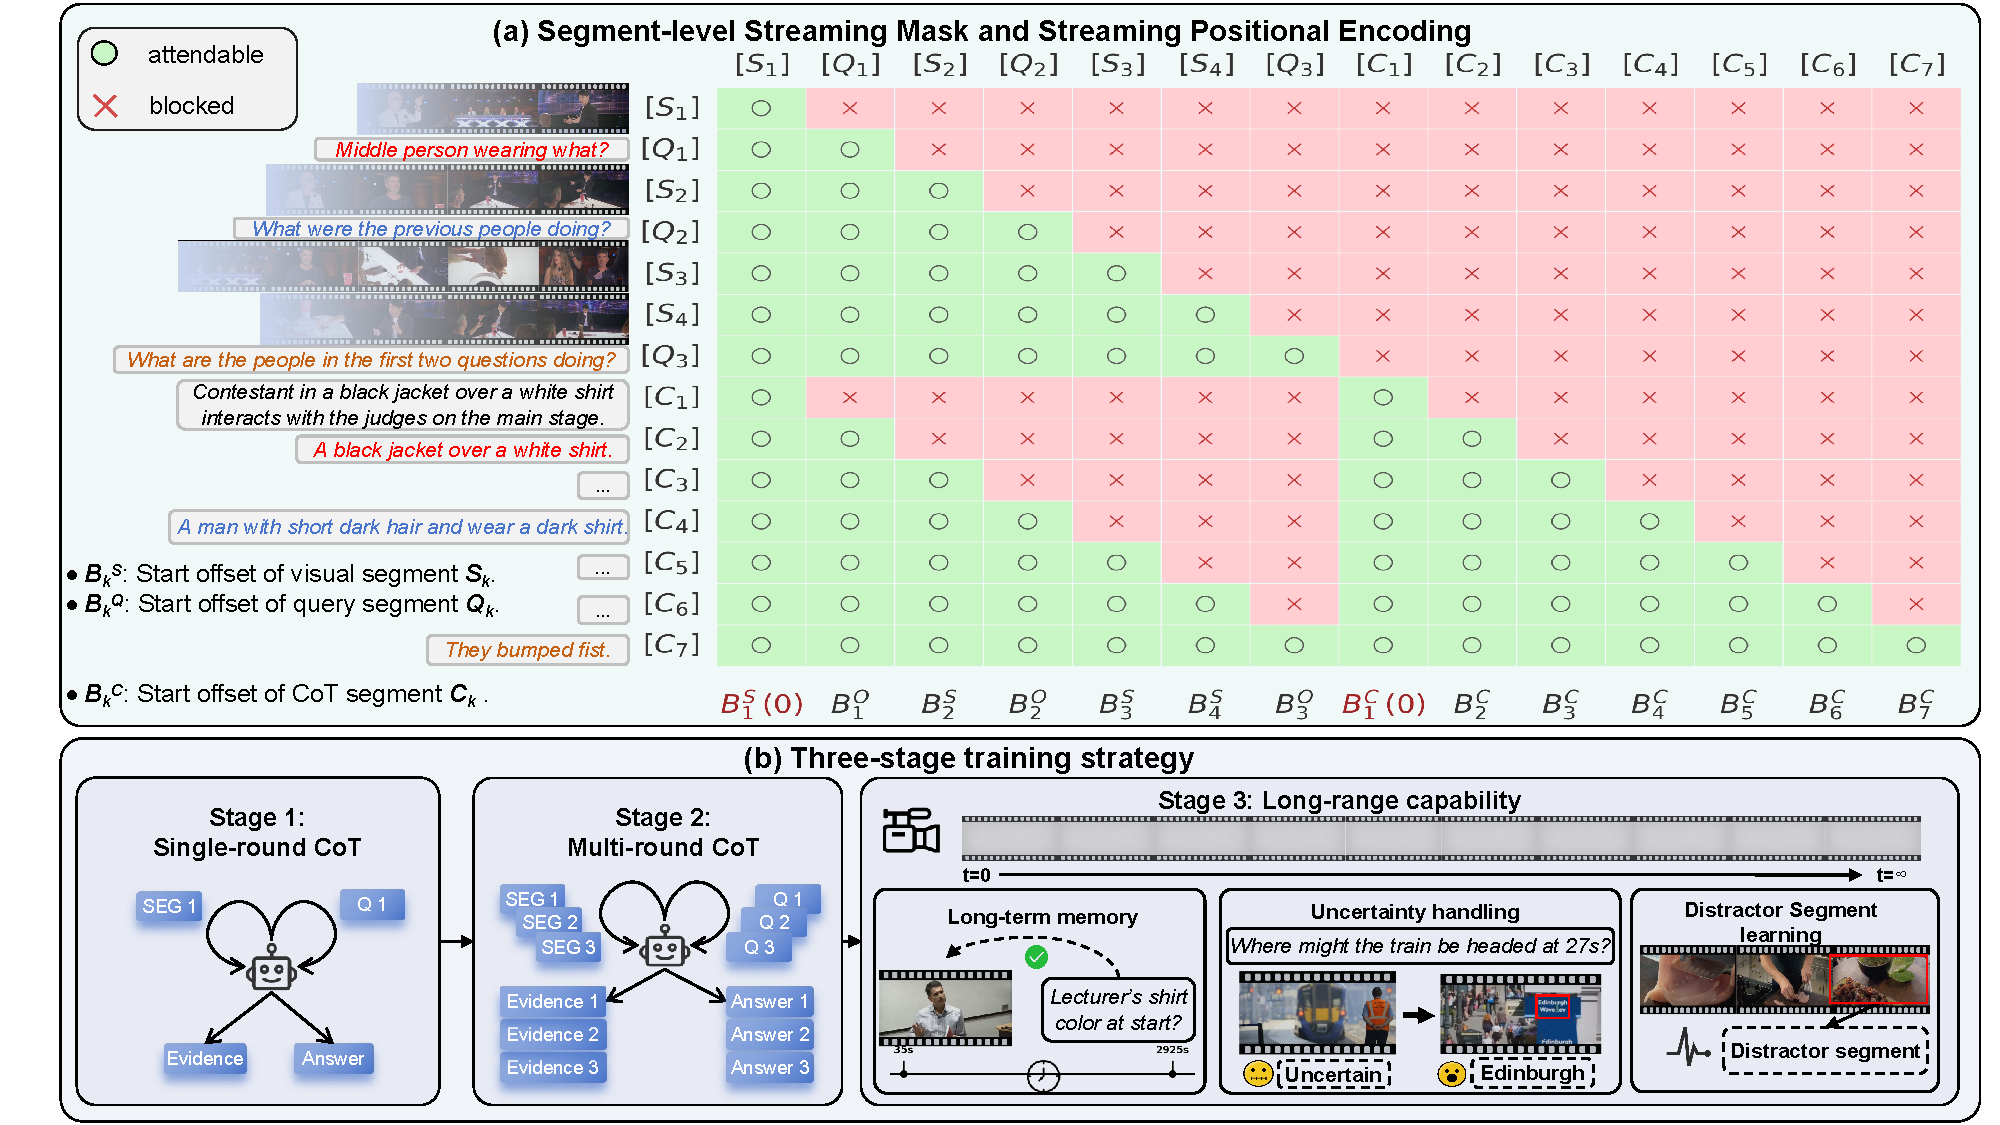
\includegraphics[width=\linewidth]{Figure/F3.pdf}
  \caption{\textbf{Training components of Think While Watching.}
  (a) segment-level streaming attention mask and streaming positional encoding: example input stream $\mathbf{R}=\langle S_1,Q_1,S_2,Q_2,S_3,S_4,Q_3\rangle$ with generated outputs $\mathbf{C}=\langle C_1,\ldots,C_7\rangle$. Green indicates the source prefix available at time step $u$, which $C_u$ is allowed to attend to. Red masks all future segments to prevent information leakage. For positional encoding, we use separate position indices for the input and output streams.
  (b) Three-stage training strategy: single-round CoT for streaming input adaptation, multi-round CoT for multi-turn interaction, and long-range capability training for long-term memory, uncertainty handling, and distractor learning.}
  \label{fig:train}
\end{figure*}

A simple streaming design interleaves perception and generation but is inherently serial: autoregressive decoding halts further input ingestion, and the interleaving pattern mismatches the LLM pretraining format. Think While Watching generates segment-level memory notes online and decouples perception and generation, enabling interaction in real time across multiple turns. Details are shown in Fig.~\ref{fig:train}.

\subsection{Segment-level Memory Notes}
\label{sec:method:memory}

To mitigate Memory Erosion, our method maintains a persistent segment-level memory bank as the online state for multi-turn streaming. For each arriving segment $\mathbf{S}_t$, the model writes exactly one memory note and appends it to the bank. The memory bank after observing the segment prefix $\mathbf{S}_{1:t}$ is defined as
\begin{equation}
\mathcal{M}_t \triangleq \{\langle i, m_i\rangle\}_{i=1}^{t}.
\end{equation}
Each note $m_t$ is a compact text unit grounded in $\mathbf{S}_t$ that records reusable evidence, including key entities and attributes, salient actions and interactions, scene changes, and short-range temporal relations. We denote the memory-writing function implemented by the MLLM backbone with parameters $\theta$ as $\mathrm{Mem}_\theta[\cdot]$, and write
\begin{equation}
m_t = \mathrm{Mem}_\theta[\mathbf{S}_t],
\qquad
C_{\operatorname{idx}[S_t]} = m_t .
\end{equation}

\noindent When a question $q_r$ is issued after observing segment $\tau_r$, the model answers by conditioning on the current question, the dialogue history, and the available memory prefix, while letting attention implicitly select relevant notes:
\begin{equation}
\langle \pi_r, a_r\rangle \sim
p_\theta\!\left[\pi_r, a_r \mid q_r, \mathcal{H}_{r-1}, \mathcal{M}_{\tau_r}\right].
\end{equation}

\subsection{Streaming Architecture}
\label{sec:method:train}

\noindent\textbf{Prefix and suffix formatting.}
To match the standard SFT format of LLMs, we serialize each training example as a source prefix followed by a target suffix. The source prefix contains the entire received unit stream $\mathbf{R}_{1:U}$, while the target suffix contains the aligned generated stream $\mathbf{C}_{1:U}$. Without additional constraints, this serialization would leak future received units to earlier generated units.

\noindent\textbf{Segment-level streaming attention mask.}
We feed the concatenated sequence
$\langle R_1,\ldots,R_U,\, C_1,\ldots,C_U\rangle$ with a segment-level mask $M^{\mathrm{seg}}$ to enforce streaming causality. Let $A$ denote the segment that contributes query tokens and $B$ denote the segment that contributes key and value tokens, with
$A,B \in \{R_1,\ldots,R_U,C_1,\ldots,C_U\}$.
The mask is defined as:
\begin{equation}
M^{\mathrm{seg}}\lbrack A,B\rbrack=
\begin{cases}
\mathbb{I}\lbrack v \le u\rbrack, & A=R_u,\; B=R_v,\\
\mathbb{I}\lbrack v \le u\rbrack, & A=C_u,\; B=R_v,\\
\mathbb{I}\lbrack k \le u\rbrack, & A=C_u,\; B=C_k,\\
0, & \text{otherwise.}
\end{cases}
\label{eq:seg-mask}
\end{equation}
Here $u$ is the arrival index of the querying unit $A$. For the attended unit $B$, we use $v$ if $B$ is a received unit $R_v$ and $k$ if $B$ is a generated unit $C_k$. The first three cases in Eq.~\eqref{eq:seg-mask} enforce streaming causality: the received stream is causal in arrival order, each generated unit $C_u$ can attend to the received prefix up to step $u$, and generated units are causal with access only to $C_{1:u}$. All remaining connections are masked, including $R_u \rightarrow C_k$ and $C_u \rightarrow R_v$ for $v>u$. We obtain token-level masks by expanding $M^{\mathrm{seg}}$ and applying standard causal masking within each $C_u$. As shown in Fig.~\ref{fig:train}(a), $C_1$ attends only to $S_1$, $C_2$ attends to $\langle S_1,Q_1\rangle$, and $C_3$ attends to $\langle S_1,Q_1,S_2\rangle$.

\noindent\textbf{Streaming positional encoding with MRoPE.}
We build on Multimodal Rotary Positional Embeddings MRoPE~\cite{DBLP:journals/corr/abs-2409-12191}, but decouple the input and output to support parallel reasoning. Specifically, the input stream follows the standard cumulative offset scheme, while the output stream independently starts positional encoding from $0$. We use $B$ to represent the base offset and compute the start offsets of the $k$-th visual segment $S_k$ input, the $k$-th question $Q_k$ input, and the $k$-th generated unit $C_k$ output:
\begin{equation}
\label{eq:stream-mrope}
B_k =
\left\{
\begin{aligned}
B_k^{S} &= \sum_{u < \operatorname{idx}\!\left[ S_k \right]} \Delta\!\left[ R_u \right],\\
B_k^{Q} &= \sum_{u < \operatorname{idx}\!\left[ Q_k \right]} \Delta\!\left[ R_u \right],\\
B_k^{C} &=
\begin{cases}
0, & k=1,\\
\sum_{i=1}^{k-1} L\!\left[ C_i \right], & k\ge 2.
\end{cases}
\end{aligned}
\right.
\end{equation}

\noindent In this design, $B_k^{S}$ and $B_k^{Q}$ are computed only from the received input prefix, while $B_k^{C}$ is computed only from previously generated tokens. Therefore, even when the output length is still unknown during decoding, newly arriving input segments can always be assigned correct input positions.\footnote{MRoPE extends RoPE to multimodal tokens by applying rotary positional encoding along modality-specific axes. For a visual segment unit $S_k$ with token grid size $\langle T_k,H_k,W_k\rangle$, a token at local grid coordinate $\langle t,h,w\rangle$ is assigned global coordinates $\langle t+B_k^{S},\,h+B_k^{S},\,w+B_k^{S}\rangle$, where the start offset $B_k^{S}$ is given in Eq.~\eqref{eq:stream-mrope}. For a text unit $Y\in\{Q_k,C_k\}$ with length $L[Y]$, a token at local position $n$ uses $n+B_k^{Q}$ for question inputs and $n+B_k^{C}$ for generated outputs. The contribution of each received unit to the input position budget is determined by the unit span $\Delta[R_u]$ in Eq.~\eqref{eq:delta}.}

\subsection{Streaming Training}
\label{sec:method:data}

\noindent\textbf{Three-stage training.}
We fine-tune the MLLM in three stages: Stage~1 learns to write segment-level memory notes and answer single-round queries. Stage~2 scales to multi-round dialogues. Stage~3 targets long-range behaviors on long videos, including long-term evidence recall, uncertainty handling, and distractor segment learning where we insert irrelevant frames as distractors. In Fig.~\ref{fig:train}(b), Stage~3 covers three long-horizon behaviors: \textbf{long-term memory} for recalling early evidence in late queries, \textbf{uncertainty handling} for deferring commitment when evidence is not yet observable, and \textbf{distractor robustness} for ignoring irrelevant segments during streaming.

\noindent\textbf{Three-stage Streaming CoT Dataset Generation.}
Streaming CoT \cite{DBLP:journals/corr/abs-2510-25332} datasets for MLLMs are extremely scarce. Multi-round streaming CoT with memory notes is largely absent. We therefore synthesize a three-stage dataset that matches our three-stage training.

\noindent\textbf{Stage 1 and Stage 2 short video streaming CoT.}
We use VideoChatOnline-IT \cite{huang2024online} as the source pool and sample up to 64 frames per instance. Stage~1 constructs 5,160 single-round instances from temporal perception subsets. Stage~2 converts 8,513 short video QA instances into 2,752 multi-round dialogues by grouping questions over the same video prefix. For both stages, we use GPT-5.2 to generate memory-anchored CoT based on the original dataset QAs.

\noindent\textbf{Stage 3 long-range streaming CoT.}
We collect long videos from YouTube using 500 keywords spanning three categories: tutorial for procedural content, lecture for explanatory content, and longform for continuous recordings. We then generate 1,500 long video instances with balanced input lengths of 100 to 200 frames, 200 to 300 frames, and 300 or more frames, and each instance contains 3 to 5 rounds. QA and CoT generation follow the same procedure as in Stage~1 and Stage~2. Details of the dataset and the prompt can be found in Appendix~\ref{app:data}.

\noindent\textbf{Quality inspection.}
We enforce the core constraints in Table~\ref{tab:prompt-constraints} during synthesis, and additionally verify that each example contains exactly $S+Q$ output items.

\begin{table}[t]
\caption{\textbf{Dataset statistics across three training stages.} Stages 1\&2 are built from VideoChatOnline-IT short videos, while Stage~3 contains long-range multi-round dialogues from YouTube. Video duration is reported in seconds (min/avg/max).}
\label{tab:data}
\centering
\scriptsize
\setlength{\tabcolsep}{3.5pt}
\renewcommand{\arraystretch}{1.05}
\resizebox{\linewidth}{!}{
\begin{tabular}{@{}lcccccccc@{}}
\toprule
\textbf{Stage} & \textbf{Source} & \textbf{Instances} & \textbf{Rounds} & \textbf{Avg. rounds} & \textbf{Frames} & \textbf{Min (s)} & \textbf{Avg (s)} & \textbf{Max (s)} \\
\midrule
1 & VideoChatOnline-IT & 5,160 & 5,160 & 1.00 & $\le 64$ & 8.18 & 79.40 & 3550.10 \\
2 & VideoChatOnline-IT & 2,752 & 8,513 & 3.09 & $\le 64$ & 2.00 & 400.92 & 3443.97 \\
3 & YouTube & 1,500 & 6,000 & 4.00 & 100-300+ & 600.12 & 1697.30 & 3595.03 \\
\bottomrule
\end{tabular}}
\end{table}

\subsection{Streaming Inference}
\label{sec:method:infer}

\noindent\textbf{Parallel reasoning.}
For real-time deployment, we adopt a dual KV cache implementation that decouples continuous source ingestion from autoregressive decoding. This engineering pattern is common in recent streaming systems \cite{DBLP:journals/corr/abs-2510-17238}. Meanwhile, we keep the same segment-level streaming mask and streaming MRoPE at inference time to ensure consistency with training.

\noindent\textbf{Adaptive attention backend.}
During decoding, our streaming mask is not always a standard causal mask: queries must attend to an allowed source prefix while remaining causal over the generated suffix, so the query and key lengths can differ ($q_{\text{len}} \neq k_{\text{len}}$). We therefore choose the attention backend adaptively---using Flash Attention \cite{dao2022flashattentionfastmemoryefficientexact} when the pattern is standard causal, and otherwise applying an explicit streaming mask with memory-efficient attention \cite{rabe2022selfattentiondoesneedon2}. Specifically, we use Flash Attention for source prefilling ($q_{\text{len}} = k_{\text{len}}$) and for autoregressive steps ($q_{\text{len}} = 1$), and switch to memory-efficient attention when $1 < q_{\text{len}} < k_{\text{len}}$ to enforce the custom streaming mask. This preserves segment-level causality while keeping inference fast.

\section{Experiments}
\label{sec:experiments}

\subsection{Datasets and Setup}
\label{sec:exp_setup}

We evaluate online streaming performance on StreamingBench~\cite{lin2024streamingbenchassessinggapmllms} and OVO-Bench~\cite{DBLP:conf/cvpr/NiuLMGZHDDD0ZZC25}. StreamingBench focuses on streaming video understanding and includes four subsets. OVO-Bench emphasizes real-world video understanding under three subsets. More details of datasets are in Appendix~\ref{app:data}.

\noindent\textbf{Evaluation protocols.}
We evaluate models under both offline and online protocols. In the offline protocol, we adopt a Batch setting where all sampled frames from the entire video are provided as a single input, and the model answers the question after observing the complete video. In the online protocol, we consider single-turn and multi-turn interaction. For single-turn online evaluation, we segment each video according to the question timestamps provided by the benchmark, forming consecutive temporal segments $[0,t_1]$, $[t_1,t_2]$, and so on. If any segment lasts longer than $60$s, we further split it into $30$s chunks. For multi-turn evaluation, we use the same segmentation strategy, but the model must answer multiple questions online as segments continuously arrive.

\noindent\textbf{Backbones and checkpoints.}
We evaluate our method with Qwen3-VL backbones at 2B, 4B, and 8B scales. We use the Instruct model for training and compare its performance with the Thinking model. TWW is used to denote our method in the following. Stage~2 and Stage~3 refer to the checkpoints obtained after training up to the second and third stages.

\subsection{Baselines}
\label{sec:exp_baselines}

\noindent\textbf{Offline evaluation.}
We evaluate Gemini 1.5 Pro \cite{geminiteam2024gemini15unlockingmultimodal} and GPT-4o \cite{openai2024gpt4ocard} as representative closed-source MLLMs. Qwen3-VL-Instruct and Qwen3-VL-Thinking are used as open-source baselines. We also report results for our TWW$_{\text{Batch,S2}}$ and TWW$_{\text{Batch,S3}}$ checkpoints, corresponding to Stage~2 and Stage~3, evaluated under the offline batch protocol.

\noindent\textbf{Online evaluation.}
For online evaluation, Instruct$_{\text{online}}$ and Thinking$_{\text{online}}$ run Qwen3-VL-Instruct and Qwen3-VL-Thinking, respectively, under the multi-turn protocol in Sec.~\ref{sec:exp_setup}. We further evaluate our checkpoints under streaming settings: TWW$_{\text{single-turn,S2}}$ and TWW$_{\text{single-turn,S3}}$ follow the single-round streaming protocol, while TWW$_{\text{multi-turn,S2}}$ and TWW$_{\text{multi-turn,S3}}$ follow the multi-round streaming protocol. Finally, Interleaved alternates between ingesting one segment and decoding text, coupling perception and generation as a naive streaming baseline. More online baselines and details are in Appendix~\ref{app:baselines}.

\subsection{Metrics}
\label{sec:exp_metrics}

We use accuracy to evaluate performance on each benchmark and each evaluation regime. We also report Avg Tokens, the average number of generated output tokens per query. Token Reduce, denoted by $\Delta$\%, is the percentage reduction of Avg Tokens compared with the Thinking baseline of the same backbone size, and Avg Frames, the average number of processed frames per query. For latency, we report TTFT, time to first token, measured as the number of tokens processed before the first answer token is produced.

\subsection{Main Results}
\label{sec:exp_main}

\Cref{tab:streamingbench_main,tab:ovobench_main} report results on two streaming benchmarks, StreamingBench and OVO-Bench. We summarize the key findings below.

\begin{enumerate}[label=\textbf{\arabic*.}]
  \item \textbf{Naive streaming inference collapses without streaming-aligned training, highlighting the difficulty of multi-turn streaming.} On StreamingBench, directly running Instruct$_{\text{online}}$ and Thinking$_{\text{online}}$ achieves only 21.47\% and 18.13\% overall, compared with 56.67\% and 58.52\% with Qwen3-VL-4B in the offline batch setting. A similar drop is observed on OVO-Bench: 21.45\% and 16.21\% versus 50.32\% and 50.70\%, showing that multi-turn streaming is nontrivial and requires streaming-aligned supervision.

  \item \textbf{Streaming-aligned supervision improves accuracy.} With Qwen3-VL-4B, TWW$_{\text{single-turn,S3}}$ improves overall accuracy from 58.52\% to 60.04\% on StreamingBench and from 50.70\% to 55.02\% on OVO-Bench compared with the Thinking baseline.

  \item \textbf{Long-video training strengthens streaming behavior.} Stage~3 generally improves upon Stage~2. For example, on OVO-Bench with the 4B backbone, TWW$_{\text{single-turn,S3}}$ improves from 54.51\% to 55.02\%.

  \item \textbf{Multi-turn segment-level memory yields a strong accuracy--efficiency tradeoff.} Under the multi-turn protocol, TWW$_{\text{multi-turn,S3}}$ maintains competitive accuracy while substantially reducing decoding tokens. With the 4B backbone, it achieves 57.40\% on StreamingBench with an average of 302.56 tokens, reducing token usage by 56.10\%. On OVO-Bench, it obtains 51.80\% with 255.91 tokens on average, reducing token usage by 45.80\%.
\end{enumerate}
We further analyzed the types of errors in Appendix~\ref{app:error}.
% ===== preamble =====

\definecolor{TabHeader}{HTML}{D9E4F2}   % 仅列名行
\definecolor{TabGroup}{HTML}{EEF2F7}    % 分组条
\definecolor{TabOffline}{HTML}{F4EEF9}  % Batch,S3：淡紫
\definecolor{TabSingle}{HTML}{EAF4FF}   % single-turn,S3：淡蓝
\definecolor{TabMulti}{HTML}{EAF8F1}    % multi-turn,S3：淡绿

\newcommand{\offc}[1]{\cellcolor{TabOffline}{#1}}
\newcommand{\sinc}[1]{\cellcolor{TabSingle}{#1}}
\newcommand{\mulc}[1]{\cellcolor{TabMulti}{#1}}

% ===== table =====
\begin{table*}[t]
\caption{\textbf{StreamingBench results} with accuracy. Columns left of the double bar report \textbf{performance}, higher is better, while columns on the right report \textbf{efficiency} for open-source models only. $\Delta$ is computed against the same backbone Thinking baseline. Avg Frames is 148.35 for the single-turn protocol and 62.58 for the multi-turn protocol.}
\label{tab:streamingbench_main}
\centering
\scriptsize
\setlength{\tabcolsep}{3.0pt}
\renewcommand{\arraystretch}{1.11}
\resizebox{\textwidth}{!}{
\begin{tabular}{@{}llcccccc||cc@{}}
\toprule
& & \multicolumn{6}{c||}{\textbf{Performance}} & \multicolumn{2}{c}{\textbf{Efficiency}} \\
\cmidrule(lr){3-8}\cmidrule(lr){9-10}
\rowcolor{TabHeader}
\textbf{Regime} & \textbf{Method} &
\textbf{SQA}$\uparrow$ & \textbf{OmniSource}$\uparrow$ & \textbf{Realtime}$\uparrow$ & \textbf{Proactive}$\uparrow$ &
\textbf{Overall}$\uparrow$ & \textbf{$\Delta$}$\uparrow$ &
\textbf{Avg Tokens}$\downarrow$ & \textbf{Token Reduce}$\uparrow$ \\
\midrule

\rowcolor{TabGroup}
\multicolumn{10}{c}{\textbf{Closed-source models}} \\
\midrule
\multirow{2}{*}{Offline}
& Gemini 1.5 Pro\cite{geminiteam2024gemini15unlockingmultimodal} & 54.80 & 67.80 & 77.39 & 45.10 & 70.26 & - & - & - \\
& GPT-4o\cite{openai2024gpt4ocard} & 32.80 & 50.95 & 74.54 & 56.86 & 64.10 & - & - & - \\
\midrule

\rowcolor{TabGroup}
\multicolumn{10}{c}{\textbf{Open-source models}} \\
\midrule
\multirow{4}{*}{Online}
& Flash-VStream-7B\cite{DBLP:journals/corr/abs-2506-23825} & 26.80 & 26.00 & 23.23 & 1.96 & 24.04 & - & - & - \\
& VideoLLM-online-8B\cite{DBLP:conf/cvpr/ChenLWLSGLGMS24} & 30.80 & 28.45 & 35.99 & 3.92 & 32.48 & - & - & - \\
& Dispider-7B\cite{DBLP:conf/cvpr/0001DD0ZCL025} & 34.80 & 35.66 & 67.63 & 25.34 & 53.12 & - & - & - \\
& StreamAgent-7B\cite{DBLP:journals/corr/abs-2508-01875} & 39.60 & 36.26 & 74.28 & 28.90 & 57.02 & - & - & - \\
\midrule

\rowcolor{TabGroup}
\multicolumn{10}{c}{\textbf{Qwen3-VL-2B}} \\
\midrule
\multirow{4}{*}{Offline}
& Instruct & 37.60 & 31.60 & 68.36 & 29.60 & 52.24 & -1.17 & - & - \\
& Thinking & 34.00 & 31.73 & 70.02 & \textbf{36.80} & 53.41 & +0.00 & 1232.91 & 0.00 \\
& TWW$_{\text{Batch,S2}}$ & 44.00 & 33.13 & 69.16 & 33.20 & 53.75 & +0.34 & 1012.35 & 17.89 \\
& \offc{\textbf{TWW$_{\text{Batch,S3}}$}}
& \offc{\textbf{44.80}}
& \offc{\textbf{33.20}}
& \offc{\textbf{69.20}}
& \offc{36.00}
& \offc{\textbf{54.00}}
& \offc{\textbf{+0.59}}
& \offc{1102.34}
& \offc{10.59} \\
\midrule
\multirow{6}{*}{Online}
& Instruct$_{\text{online}}$ & 9.20 & 28.80 & 21.28 & 13.20 & 22.67 & -30.74 & - & - \\
& Thinking$_{\text{online}}$ & 8.40 & 11.60 & 12.92 & 19.20 & 12.58 & -40.83 & 832.23 & 32.50 \\
\cmidrule(lr){2-10}
& TWW$_{\text{single-turn,S2}}$ & 47.20 & 34.20 & 71.84 & 32.80 & 55.76 & +2.35 & 923.58 & 25.09 \\
& \sinc{\textbf{TWW$_{\text{single-turn,S3}}$}}
& \sinc{\textbf{48.00}}
& \sinc{\textbf{34.27}}
& \sinc{\textbf{72.00}}
& \sinc{34.40}
& \sinc{\textbf{56.00}}
& \sinc{\textbf{+2.59}}
& \sinc{930.23}
& \sinc{24.55} \\
\cmidrule(lr){2-10}
& TWW$_{\text{multi-turn,S2}}$ & 42.40 & 31.33 & 69.20 & 33.60 & 53.11 & -0.30 & \textbf{285.42} & \textbf{76.85} \\
& \mulc{\textbf{TWW$_{\text{multi-turn,S3}}$}}
& \mulc{45.20}
& \mulc{31.47}
& \mulc{69.24}
& \mulc{34.80}
& \mulc{\textbf{53.40}}
& \mulc{-0.01}
& \mulc{300.20}
& \mulc{75.65} \\
\midrule

\rowcolor{TabGroup}
\multicolumn{10}{c}{\textbf{Qwen3-VL-4B}} \\
\midrule
\multirow{4}{*}{Offline}
& Instruct & 37.20 & 38.47 & 71.36 & 38.40 & 56.67 & -1.85 & - & - \\
& Thinking & 46.40 & 36.53 & \textbf{74.50} & 42.80 & 58.52 & +0.00 & 689.22 & 0.00 \\
& TWW$_{\text{Batch,S2}}$ & 42.40 & 39.60 & 71.84 & 39.60 & 57.67 & -0.85 & 594.28 & 13.77 \\
& \offc{\textbf{TWW$_{\text{Batch,S3}}$}}
& \offc{44.00}
& \offc{\textbf{39.67}}
& \offc{71.88}
& \offc{40.80}
& \offc{57.87}
& \offc{-0.65}
& \offc{620.35}
& \offc{9.99} \\
\midrule
\multirow{6}{*}{Online}
& Instruct$_{\text{online}}$ & 12.80 & 21.53 & 22.88 & 15.60 & 21.47 & -37.05 & - & - \\
& Thinking$_{\text{online}}$ & 21.20 & 21.47 & 16.92 & 7.20 & 18.13 & -40.39 & 482.24 & 30.03 \\
\cmidrule(lr){2-10}
& TWW$_{\text{single-turn,S2}}$ & 46.00 & 40.67 & 74.36 & 41.20 & 59.71 & +1.19 & 558.12 & 19.02 \\
& \sinc{\textbf{TWW$_{\text{single-turn,S3}}$}}
& \sinc{\textbf{46.80}}
& \sinc{\textbf{41.00}}
& \sinc{74.48}
& \sinc{\textbf{43.20}}
& \sinc{\textbf{60.04}}
& \sinc{\textbf{+1.52}}
& \sinc{570.68}
& \sinc{17.20} \\
\cmidrule(lr){2-10}
& TWW$_{\text{multi-turn,S2}}$ & 40.80 & 39.20 & 71.20 & 40.00 & 57.11 & -1.41 & \textbf{291.86} & \textbf{57.65} \\
& \mulc{\textbf{TWW$_{\text{multi-turn,S3}}$}}
& \mulc{43.60}
& \mulc{39.33}
& \mulc{71.28}
& \mulc{40.80}
& \mulc{\textbf{57.40}}
& \mulc{-1.12}
& \mulc{302.56}
& \mulc{56.10} \\
\midrule

\rowcolor{TabGroup}
\multicolumn{10}{c}{\textbf{Qwen3-VL-8B}} \\
\midrule
\multirow{4}{*}{Offline}
& Instruct & 44.40 & 37.53 & 73.60 & 36.00 & 57.87 & -0.35 & - & - \\
& Thinking & 45.60 & 35.47 & 74.46 & \textbf{44.80} & 58.21 & +0.00 & 759.30 & 0.00 \\
& TWW$_{\text{Batch,S2}}$ & 52.80 & 38.93 & 74.56 & 38.00 & 59.44 & +1.23 & 708.16 & 6.70 \\
& \offc{\textbf{TWW$_{\text{Batch,S3}}$}}
& \offc{\textbf{53.20}}
& \offc{\textbf{39.07}}
& \offc{\textbf{74.64}}
& \offc{40.00}
& \offc{\textbf{59.67}}
& \offc{\textbf{+1.45}}
& \offc{720.30}
& \offc{5.10} \\
\midrule
\multirow{6}{*}{Online}
& Instruct$_{\text{online}}$ & 17.20 & 21.47 & 25.12 & 17.60 & 23.04 & -35.17 & - & - \\
& Thinking$_{\text{online}}$ & 14.80 & 13.00 & 17.56 & 16.40 & 15.82 & -42.39 & 573.75 & 24.41 \\
\cmidrule(lr){2-10}
& TWW$_{\text{single-turn,S2}}$ & 54.00 & 40.07 & 77.60 & 39.60 & 61.67 & +3.46 & 651.74 & 14.13 \\
& \sinc{\textbf{TWW$_{\text{single-turn,S3}}$}}
& \sinc{\textbf{54.40}}
& \sinc{\textbf{40.67}}
& \sinc{\textbf{77.68}}
& \sinc{41.60}
& \sinc{\textbf{62.04}}
& \sinc{\textbf{+3.83}}
& \sinc{660.92}
& \sinc{12.92} \\
\cmidrule(lr){2-10}
& TWW$_{\text{multi-turn,S2}}$ & 48.80 & 37.40 & 74.32 & 38.40 & 58.60 & +0.39 & \textbf{288.64} & \textbf{61.97} \\
& \mulc{\textbf{TWW$_{\text{multi-turn,S3}}$}}
& \mulc{50.00}
& \mulc{37.47}
& \mulc{74.40}
& \mulc{40.00}
& \mulc{\textbf{58.82}}
& \mulc{+0.61}
& \mulc{290.82}
& \mulc{61.68} \\
\bottomrule
\end{tabular}}
\end{table*}

\begin{table*}[!h]
\caption{\textbf{OVO-Bench results}. Avg Frames is 63.23 for the single-turn protocol and 25.47 for the multi-turn protocol.}
\label{tab:ovobench_main}
\centering
\scriptsize
\setlength{\tabcolsep}{2.8pt}
\renewcommand{\arraystretch}{1.11}
\resizebox{\textwidth}{!}{
\begin{tabular}{@{}llccccc||cc@{}}
\toprule
& & \multicolumn{5}{c||}{\textbf{Performance}} & \multicolumn{2}{c}{\textbf{Efficiency}} \\
\cmidrule(lr){3-7}\cmidrule(lr){8-9}
\rowcolor{TabHeader}
\textbf{Regime} & \textbf{Method} &
\textbf{Backward}$\uparrow$ & \textbf{Realtime}$\uparrow$ & \textbf{Forward}$\uparrow$ & \textbf{Overall}$\uparrow$ & \textbf{$\Delta$}$\uparrow$ &
\textbf{Avg Tokens}$\downarrow$ & \textbf{Token Reduce}$\uparrow$ \\
\midrule

\rowcolor{TabGroup}
\multicolumn{9}{c}{\textbf{Closed-source models}} \\
\midrule
\multirow{2}{*}{Offline}
& Gemini 1.5 Pro\cite{geminiteam2024gemini15unlockingmultimodal} & 69.32 & 62.54 & 57.15 & 63.00 & - & - & - \\
& GPT-4o\cite{openai2024gpt4ocard} & 64.46 & 60.75 & 53.40 & 59.54 & - & - & - \\
\midrule

\rowcolor{TabGroup}
\multicolumn{9}{c}{\textbf{Open-source models}} \\
\midrule
\multirow{4}{*}{Online}
& Flash-VStream-7B\cite{DBLP:journals/corr/abs-2506-23825} & 27.38 & 28.37 & 45.09 & 33.61 & - & - & - \\
& Dispider-7B\cite{DBLP:conf/cvpr/0001DD0ZCL025} & 36.06 & 54.55 & 34.72 & 41.78 & - & - & - \\
& StreamForest-7B\cite{DBLP:journals/corr/abs-2509-24871} & 52.02 & 61.20 & 53.49 & 55.57 & - & - & - \\
& StreamAgent-7B\cite{DBLP:journals/corr/abs-2508-01875} & 41.70 & 61.30 & 45.40 & 49.40 & - & - & - \\
\midrule

\rowcolor{TabGroup}
\multicolumn{9}{c}{\textbf{Qwen3-VL-2B}} \\
\midrule
\multirow{4}{*}{Offline}
& Instruct & 37.29 & 56.65 & \textbf{51.51} & 49.97 & +2.23 & - & - \\
& Thinking & 41.78 & 57.27 & 45.04 & 47.74 & +0.00 & 590.25 & 0.00 \\
& TWW$_{\text{Batch,S2}}$ & 43.25 & 56.52 & 44.72 & 47.67 & -0.07 & 518.64 & 12.13 \\
& \offc{\textbf{TWW$_{\text{Batch,S3}}$}}
& \offc{44.37}
& \offc{56.87}
& \offc{45.31}
& \offc{48.30}
& \offc{\textbf{+0.56}}
& \offc{530.32}
& \offc{10.15} \\
\midrule
\multirow{6}{*}{Online}
& Instruct$_{\text{online}}$ & 11.89 & 16.01 & 26.87 & 20.76 & -26.98 & - & - \\
& Thinking$_{\text{online}}$ & 8.56 & 19.47 & 20.29 & 17.63 & -30.11 & 478.74 & 18.89 \\
\cmidrule(lr){2-9}
& TWW$_{\text{single-turn,S2}}$ & 44.58 & 57.85 & 47.35 & 49.67 & +1.93 & 456.28 & 22.70 \\
& \sinc{\textbf{TWW$_{\text{single-turn,S3}}$}}
& \sinc{\textbf{45.96}}
& \sinc{\textbf{58.18}}
& \sinc{47.86}
& \sinc{\textbf{50.31}}
& \sinc{\textbf{+2.57}}
& \sinc{470.20}
& \sinc{20.34} \\
\cmidrule(lr){2-9}
& TWW$_{\text{multi-turn,S2}}$ & 40.85 & 55.42 & 44.34 & 46.67 & -1.07 & \textbf{278.52} & \textbf{52.81} \\
& \mulc{\textbf{TWW$_{\text{multi-turn,S3}}$}}
& \mulc{42.16}
& \mulc{55.79}
& \mulc{44.54}
& \mulc{47.15}
& \mulc{-0.59}
& \mulc{280.32}
& \mulc{52.51} \\
\midrule

\rowcolor{TabGroup}
\multicolumn{9}{c}{\textbf{Qwen3-VL-4B}} \\
\midrule
\multirow{4}{*}{Offline}
& Instruct & 44.32 & 62.39 & 46.29 & 50.32 & -0.38 & - & - \\
& Thinking & 50.78 & 61.17 & 45.08 & 50.70 & +0.00 & 472.18 & 0.00 \\
& TWW$_{\text{Batch,S2}}$ & 52.45 & 62.18 & 47.37 & 52.51 & +1.81 & 412.37 & 12.67 \\
& \offc{\textbf{TWW$_{\text{Batch,S3}}$}}
& \offc{53.88}
& \offc{62.37}
& \offc{47.86}
& \offc{53.11}
& \offc{\textbf{+2.41}}
& \offc{430.51}
& \offc{8.83} \\
\midrule
\multirow{6}{*}{Online}
& Instruct$_{\text{online}}$ & 13.63 & 20.79 & 24.95 & 21.45 & -29.25 & - & - \\
& Thinking$_{\text{online}}$ & 14.42 & 14.10 & 18.06 & 16.21 & -34.49 & 360.63 & 23.62 \\
\cmidrule(lr){2-9}
& TWW$_{\text{single-turn,S2}}$ & 53.92 & 64.25 & 49.55 & 54.51 & +3.81 & 358.45 & 24.09 \\
& \sinc{\textbf{TWW$_{\text{single-turn,S3}}$}}
& \sinc{\textbf{55.47}}
& \sinc{\textbf{64.52}}
& \sinc{\textbf{49.78}}
& \sinc{\textbf{55.02}}
& \sinc{\textbf{+4.32}}
& \sinc{378.64}
& \sinc{19.81} \\
\cmidrule(lr){2-9}
& TWW$_{\text{multi-turn,S2}}$ & 48.65 & 60.85 & 47.67 & 51.51 & +0.81 & \textbf{251.36} & \textbf{46.77} \\
& \mulc{\textbf{TWW$_{\text{multi-turn,S3}}$}}
& \mulc{49.13}
& \mulc{61.17}
& \mulc{47.86}
& \mulc{51.80}
& \mulc{+1.10}
& \mulc{255.91}
& \mulc{45.80} \\
\midrule

\rowcolor{TabGroup}
\multicolumn{9}{c}{\textbf{Qwen3-VL-8B}} \\
\midrule
\multirow{4}{*}{Offline}
& Instruct & 42.63 & 62.86 & 51.02 & 52.54 & -1.28 & - & - \\
& Thinking & 54.24 & 61.34 & 49.63 & 53.82 & +0.00 & 390.42 & 0.00 \\
& TWW$_{\text{Batch,S2}}$ & 55.82 & 63.15 & 51.83 & 55.78 & +1.96 & 325.82 & 16.55 \\
& \offc{\textbf{TWW$_{\text{Batch,S3}}$}}
& \offc{\textbf{57.37}}
& \offc{63.68}
& \offc{52.01}
& \offc{56.34}
& \offc{\textbf{+2.52}}
& \offc{340.22}
& \offc{12.86} \\
\midrule
\multirow{6}{*}{Online}
& Instruct$_{\text{online}}$ & 15.69 & 25.57 & 21.12 & 21.22 & -32.60 & - & - \\
& Thinking$_{\text{online}}$ & 11.25 & 19.59 & 18.51 & 17.30 & -36.52 & 330.67 & 15.30 \\
\cmidrule(lr){2-9}
& TWW$_{\text{single-turn,S2}}$ & 56.45 & 64.52 & 52.78 & 56.78 & +2.96 & 276.19 & 29.26 \\
& \sinc{\textbf{TWW$_{\text{single-turn,S3}}$}}
& \sinc{57.05}
& \sinc{\textbf{64.76}}
& \sinc{52.97}
& \sinc{\textbf{57.07}}
& \sinc{\textbf{+3.25}}
& \sinc{290.07}
& \sinc{25.70} \\
\cmidrule(lr){2-9}
& TWW$_{\text{multi-turn,S2}}$ & 52.05 & 63.25 & 52.85 & 55.55 & +1.73 & \textbf{224.68} & \textbf{42.45} \\
& \mulc{\textbf{TWW$_{\text{multi-turn,S3}}$}}
& \mulc{52.77}
& \mulc{63.68}
& \mulc{\textbf{53.29}}
& \mulc{56.05}
& \mulc{+2.23}
& \mulc{227.33}
& \mulc{41.77} \\
\bottomrule
\end{tabular}}
\end{table*}

\subsection{Analysis}
\label{sec:exp_analysis}

\begin{figure}[t]
  \centering
  \begin{minipage}[t]{0.49\linewidth}
    \centering
    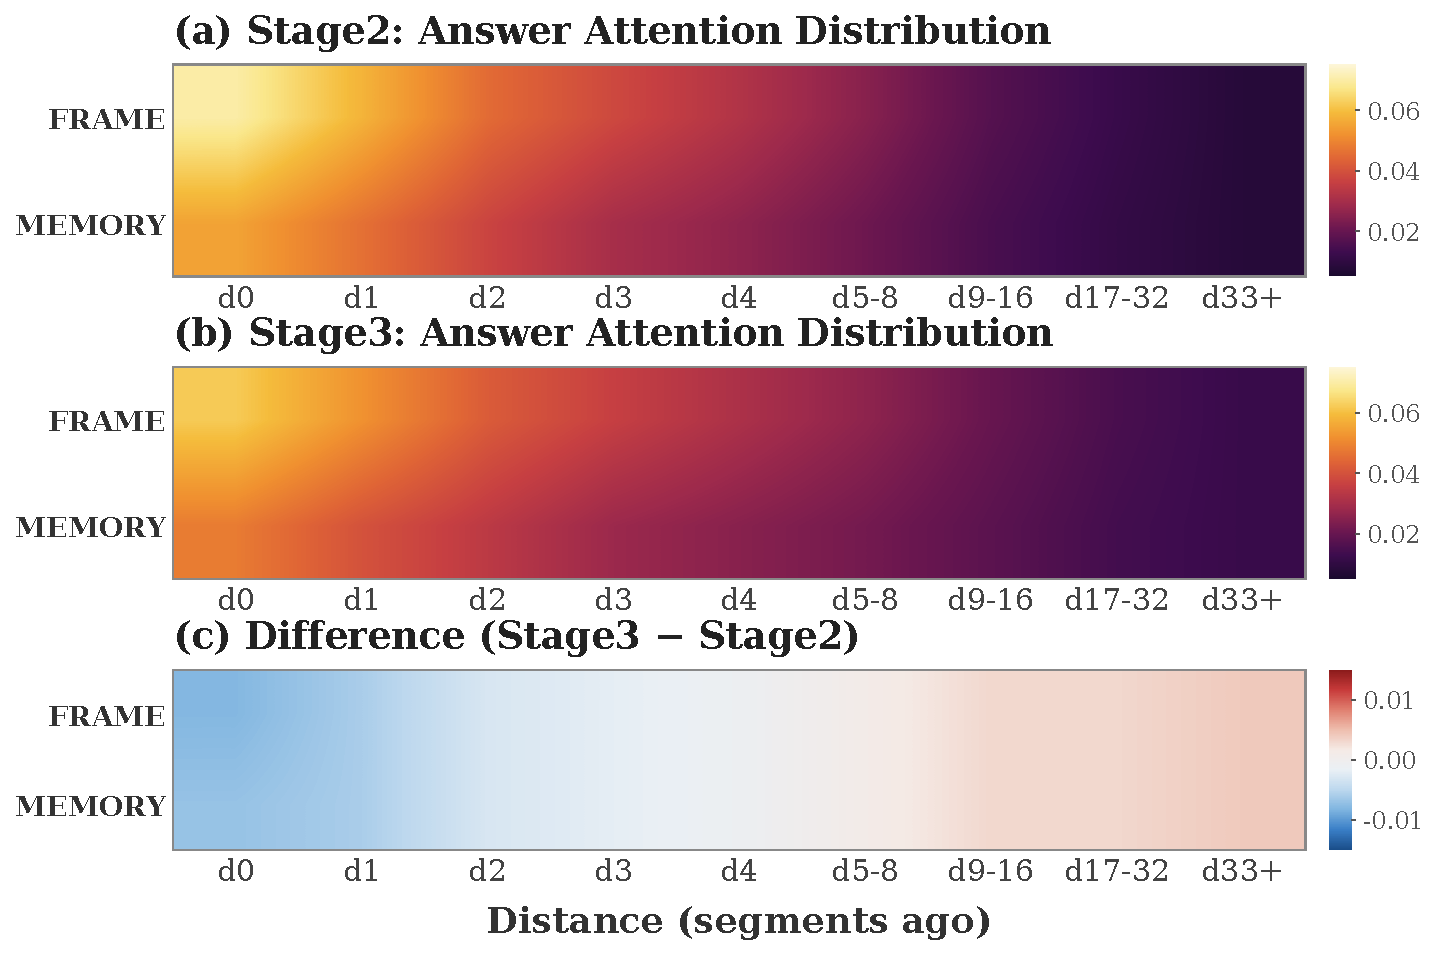
\includegraphics[width=\linewidth]{Figure/attention.pdf}
    \caption{\textbf{Answer attention vs.\ segment distance} on TWW$_{\text{multi-turn}}$. After Stage~3, attention mass shifts from near-history to more distant segments.}
    \label{fig:attn_dist}
  \end{minipage}\hfill
  \begin{minipage}[t]{0.49\linewidth}
    \centering
    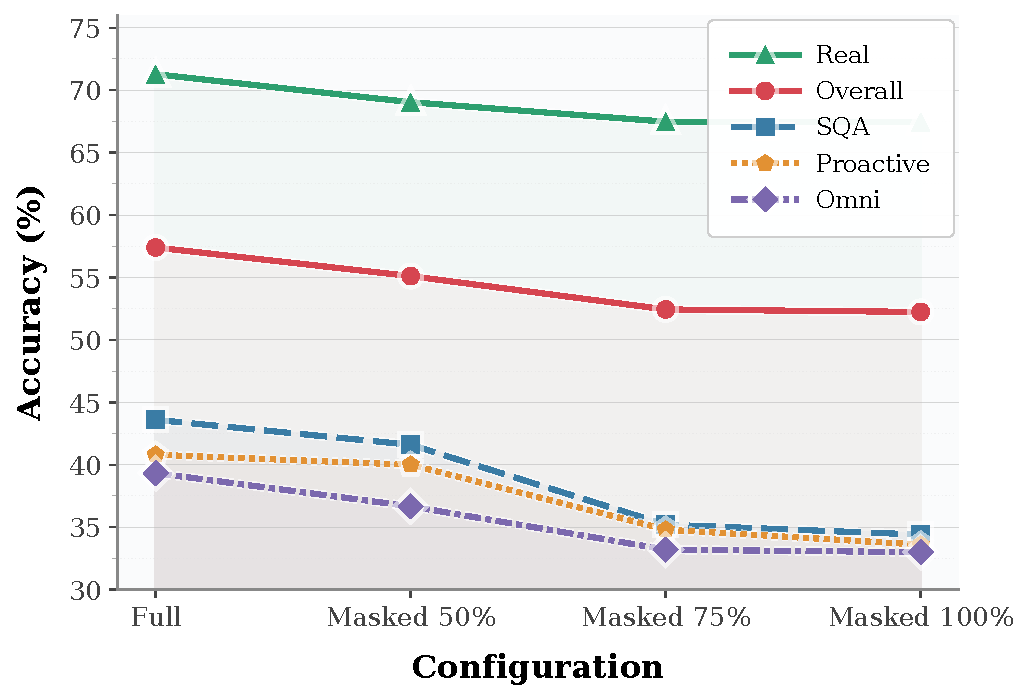
\includegraphics[width=\linewidth]{Figure/frame_mask_curve.pdf}
    \caption{\textbf{Ablation} under frame masking on TWW$_{\text{multi-turn,S3}}$. Overall represents the accuracy rate. The remaining curves represent the results of the subsets.}
    \label{fig:frame_mask}
  \end{minipage}
\end{figure}

\refstepcounter{subsubsection}
\noindent\textbf{Generalization to Offline Video Understanding.}
\label{sec:offline_generalization}
Although our training is designed for streaming scenarios, we also evaluate whether the learned behaviors can transfer to offline video understanding tasks. We evaluate on two offline benchmarks: \textbf{Video-MME}~\cite{DBLP:conf/cvpr/FuDLLRZWZSZCLLZ25} and \textbf{LV-Bench}~\cite{wang2025lvbenchextremelongvideo}, following their official evaluation settings. \Cref{tab:offline_results} shows that streaming training also benefits offline evaluation. In particular, TWW$_{\text{single-turn,S3}}$ improves Video-MME from 68.89\% to \textbf{73.41\%} and LV-Bench from 53.47\% to \textbf{57.68\%}, showing that long-range streaming supervision transfers effectively to offline long-video reasoning. Unless otherwise stated, the following analyses use Qwen3-VL-4B on StreamingBench.

\begin{table*}[t]
\caption{\textbf{Offline video understanding results} on Video-MME and LV-Bench.}
\label{tab:offline_results}
\centering
\scriptsize
\setlength{\tabcolsep}{3.0pt}
\renewcommand{\arraystretch}{1.08}
\resizebox{\textwidth}{!}{
\begin{tabular}{@{}lccccccccccc@{}}
\toprule
& \multicolumn{4}{c}{\textbf{Video-MME}} & \multicolumn{7}{c}{\textbf{LV-Bench}} \\
\cmidrule(lr){2-5} \cmidrule(lr){6-12}
\textbf{Method} & \textbf{Short} & \textbf{Medium} & \textbf{Long} & \textbf{Overall} & \textbf{ER} & \textbf{EU} & \textbf{KIR} & \textbf{TG} & \textbf{Rea} & \textbf{Sum} & \textbf{Overall} \\
\midrule
Thinking & 77.78 & 66.67 & 62.22 & 68.89 & 54.22 & 51.62 & 62.07 & 46.82 & 55.50 & 40.35 & 53.47 \\
Instruct & 78.22 & 66.78 & 62.89 & 69.30 & 56.15 & 53.78 & 65.86 & 50.45 & 60.00 & 43.86 & 56.19 \\
TWW$_{\text{Batch,S3}}$ & 78.89 & 67.11 & 64.00 & 70.00 & \textbf{58.07} & 54.24 & 66.21 & \textbf{51.36} & 62.00 & 47.37 & 57.39 \\
TWW$_{\text{multi-turn,S3}}$ & 79.00 & 67.11 & 62.33 & 69.48 & 56.44 & 54.39 & 66.55 & 50.91 & 61.50 & 45.61 & 56.81 \\
TWW$_{\text{single-turn,S3}}$ & \textbf{83.22} & \textbf{70.11} & \textbf{66.89} & \textbf{73.41} & 57.33 & \textbf{54.70} & \textbf{67.59} & \textbf{51.36} & \textbf{62.50} & \textbf{52.63} & \textbf{57.68} \\
\bottomrule
\end{tabular}}
\end{table*}

\refstepcounter{subsubsection}
\noindent\textbf{Long-Range Attention Analysis.}
\label{sec:analysis_attention}
We analyze how far back the model consults history when generating answers by aggregating the last-layer attention from answer tokens to historical tokens and grouping the attended history by segment distance $d=\tau_r-i$, where $\tau_r$ denotes the index of the latest observed segment when answering the $r$-th question, and $i\le\tau_r$ denotes the index of a historical segment being attended to. Here, $d=0$ corresponds to the most recent segment, and larger $d$ indicates segments further in the past.

We separately measure attention to \textbf{FRAME} tokens, which are visual tokens from prior segments, and \textbf{MEMORY} tokens, which are accumulated memory note tokens written for those segments. \Cref{fig:attn_dist} shows that the Stage~2 checkpoint exhibits a strong recency bias, whereas Stage~3 reallocates attention mass from near-history buckets to more distant buckets. The shift is more pronounced on \textbf{MEMORY} tokens than on visual tokens, consistent with the intended role of memory notes as a compact long-range state for multi-turn interaction.

\refstepcounter{subsubsection}
\noindent\textbf{Ablation Studies.}
\label{sec:analysis_ablation}
We conduct ablations to isolate the roles of the memory bank, visual inputs, and segmentation granularity. Removing the memory bank causes a clear accuracy drop from $57.40$\% to $52.35$\% in \Cref{tab:memory_ablation}, confirming that memory notes serve as an effective persistent state in multi-round streams. For visual ablations, Fig.~\ref{fig:frame_mask} shows a monotonic degradation as more frames are masked. Performance remains relatively stable under moderate corruption, suggesting that once written, segment-level memory notes provide a stabilizing signal. Under severe corruption, accuracy approaches the no-memory regime, which is expected because memory writing becomes unreliable without sufficient visual evidence. For segmentation granularity, Table~\ref{tab:memory_ablation} reveals a clear accuracy and efficiency tradeoff. Using longer segments $120$s/$60$s reduces the average decoding length from 302.56 to 230.46 tokens but causes a noticeable accuracy drop of $2.07$\%. Conversely, using shorter segments $30$s/$15$s preserves accuracy but increases the average decoding length to 380.50 tokens (+$25.8$\%), due to more frequent memory updates.

\begin{table}[t]
\centering
\begin{minipage}[t]{0.49\linewidth}
\centering
\captionof{table}{\textbf{Ablations} on StreamingBench. a/b represents the maximum segment duration and the chunk duration.}
\label{tab:memory_ablation}
{\scriptsize
\setlength{\tabcolsep}{4pt}
\renewcommand{\arraystretch}{1.06}
\begin{tabular}{@{}llcc@{}}
\toprule
\textbf{Category} & \textbf{Setting} & \textbf{Acc}$\uparrow$ & \textbf{Avg Tok}$\downarrow$ \\
\midrule
Memory & with notes & \textbf{57.40} & 302.56 \\
Memory & without notes & 52.35 & 330.73 \\
\midrule
Segment & $60$s/$30$s & \textbf{57.40} & 302.56 \\
Segment & $120$s/$60$s & 55.33 & \textbf{230.46} \\
Segment & $30$s/$15$s & 57.20 & 380.50 \\
\bottomrule
\end{tabular}}
\end{minipage}\hfill
\begin{minipage}[t]{0.49\linewidth}
\centering
\captionof{table}{\textbf{TTFT on StreamingBench.} Overall accuracy and time-to-first-token of Qwen3-VL-4B for batch, interleaved streaming, and our TWW$_{\text{multi-turn,S3}}$ pipeline.}
\label{tab:ttft}
{\scriptsize
\setlength{\tabcolsep}{6pt}
\renewcommand{\arraystretch}{1.06}
\begin{tabular}{@{}lcc@{}}
\toprule
\textbf{Method} & \textbf{Overall Acc}$\uparrow$ & \textbf{TTFT}$\downarrow$ \\
\midrule
Thinking & \textbf{58.52} & 31203.69 \\
Interleaved & 55.35 & \textbf{2304.28} \\
TWW$_{\text{multi-turn,S3}}$ & 57.40 & \textbf{2304.28} \\
\bottomrule
\end{tabular}}
\end{minipage}
\end{table}

\refstepcounter{subsubsection}
\noindent\textbf{TTFT Analysis.}
\label{sec:analysis_ttft}
Table~\ref{tab:ttft} reports overall accuracy and TTFT on StreamingBench with the 4B backbone. Compared with batch Thinking, our streaming pipeline reduces TTFT by \textbf{92.6\%}, from 31203.69 to 2304.28 tokens, while maintaining comparable accuracy. The interleaved baseline achieves a similar TTFT for multi-turn streaming but is consistently less accurate.

\refstepcounter{subsubsection}
\noindent\textbf{Theoretical Latency Analysis.}
\label{sec:analysis_theory_latency}
Our method decouples ingestion from decoding, largely eliminating decoder-induced ingestion backlog, thereby avoiding backlog explosion as $\rho$ (arrival rate over processing rate) approaches $1$ and significantly reducing latency. The complete derivation is in Appendix~\ref{app:latency}.

\section{Conclusion}

We presented \textbf{Think While Watching}, a memory-anchored streaming video reasoning framework for multi-turn interaction over continuously arriving streams. Our approach maintains \textbf{segment-level memory notes} as a persistent state, enforces strict causality through a \textbf{segment-level streaming causal mask} and \textbf{streaming positional encoding}, and enables practical real-time deployment via a dual KV cache pipeline with adaptive attention backends. Experiments on StreamingBench and OVO-Bench validate the proposed method’s effectiveness, consistently improving online accuracy while maintaining strong efficiency.

\bibliographystyle{unsrtnat}
\bibliography{main}

\clearpage
\appendix

\renewcommand{\thetable}{A\arabic{table}}
\renewcommand{\thefigure}{A\arabic{figure}}
\setcounter{table}{0}
\setcounter{figure}{0}

\section{Future Work}
Future work will explore adaptive segmentation that selects segment boundaries online based on scene changes and question demands, reducing redundant memory updates while preserving evidence coverage. We also plan to incorporate audio cues and speech transcripts to support richer streaming understanding in real-world settings. Another direction is improving robustness on very long streams through better uncertainty estimation, memory verification, and training with harder distractors and domain shifts. Finally, we will develop more comprehensive evaluation protocols that jointly measure accuracy, latency, and resource usage in multi-turn interaction.

\section{Implementation Details}

All experiments are conducted on 8$\times$ NVIDIA RTX A6000 GPUs (48GB each). We fine-tune Qwen3-VL-2/4/8B-Instruct using full-parameter supervised fine-tuning (SFT). Table~\ref{tab:impl_details} summarizes the main training settings.

\begin{table}[h]
\centering
\caption{Implementation details and training hyperparameters.}
\label{tab:impl_details}
\begin{tabular}{ll}
\toprule
\textbf{Item} & \textbf{Setting} \\
\midrule
GPUs & 8$\times$ NVIDIA RTX A6000 (48GB) \\
Model & Qwen3-VL-2/4/8B-Instruct \\
Training method & Full-parameter SFT \\
Precision & bf16 \\
Global batch size & 128 \\
Optimizer & AdamW \\
Peak learning rate & $1.0\times10^{-5}$ \\
Learning rate schedule & Cosine decay \\
Warmup ratio & 3\% \\
Weight decay & 0.1 \\
Stage 1 strategy & DeepSpeed ZeRO-3 \\
Gradient checkpointing & Enabled \\
Communication overlap & Enabled \\
\bottomrule
\end{tabular}
\end{table}

\section{Theoretical Latency Derivation}
\label{app:latency}

We derive a simple queueing-style model to quantify decoder-induced ingestion backlog in interleaved streaming, as illustrated in Fig.~\ref{fig:latency}.

\noindent\textbf{Stream arrival and processing rates.}
Assume that video segments arrive in real time at a rate of $\lambda$ segments per second. When the model is watching, meaning that it is ingesting and prefilling, it processes segments at a rate of $\mu$ segments per second. We define the utilization by $\rho \triangleq \lambda/\mu$.

\noindent\textbf{Interleaved decoding as server downtime.}
In the interleaved baseline, generation is non-preemptive: during a decoding period of duration $T_{\mathrm{dec}}$, the system does not ingest new segments. While decoding, the stream continues to arrive, creating a backlog of
\begin{equation}
B \;=\; \lambda\, T_{\mathrm{dec}} .
\label{eq:backlog_size}
\end{equation}
$B$ represents backlog, which refers to the number of video segments that are accumulated and yet to be processed. After decoding, the system resumes watching at rate $\mu$ while new segments still arrive at rate $\lambda$. Thus the backlog drains at a net rate $(\mu-\lambda)$ (assuming $\mu>\lambda$), and the \textbf{catch-up time} is
\begin{equation}
T_{\mathrm{catch}}
\;=\;
\frac{B}{\mu-\lambda}
\;=\;
\frac{\lambda}{\mu-\lambda}\, T_{\mathrm{dec}}
\;=\;
\frac{\rho}{1-\rho}\, T_{\mathrm{dec}} .
\label{eq:catchup_time}
\end{equation}
This yields an amplification effect: each second spent decoding induces an additional $\rho/(1-\rho)$ second of future delay before the system fully catches up, which diverges as $\rho \rightarrow 1$.

\noindent\textbf{Think While Watching weakens backlog coupling.}
Our inference design decouples ingestion from decoding via dual KV caching, so decoding no longer forces a full stop of stream ingestion as in interleaved streaming. As a result, the decoder-induced backlog is greatly reduced. In an ideal fully overlapped implementation, the additional ingestion downtime during decoding approaches zero, yielding
\begin{equation}
B_{\mathrm{ours}} \approx 0 \quad\Rightarrow\quad T_{\mathrm{catch}} \approx 0 .
\end{equation}
In practice, however, a residual backlog may still arise from system overheads such as scheduling, synchronization, cache maintenance, and time overlapping. Therefore, the main benefit of our design is not to guarantee zero backlog but to substantially reduce the coupling between decoding and future stream lag.

\noindent\textbf{A quality real-time constraint in interleaving.}
Let $c_{\mathrm{tok}}$ be the average decoding time per output token and $L$ be the number of generated tokens per step. Interleaving spends $T_{\mathrm{dec}} = c_{\mathrm{tok}}L$ during which ingestion is paused, inducing
$T_{\mathrm{catch}}=\frac{\rho}{1-\rho}c_{\mathrm{tok}}L$ by Eq.~\eqref{eq:catchup_time}. Therefore, increasing $L$ to improve quality directly increases future stream lag. Our method weakens this coupling by allowing ingestion to proceed while decoding.

\begin{figure}[h]
  \centering
  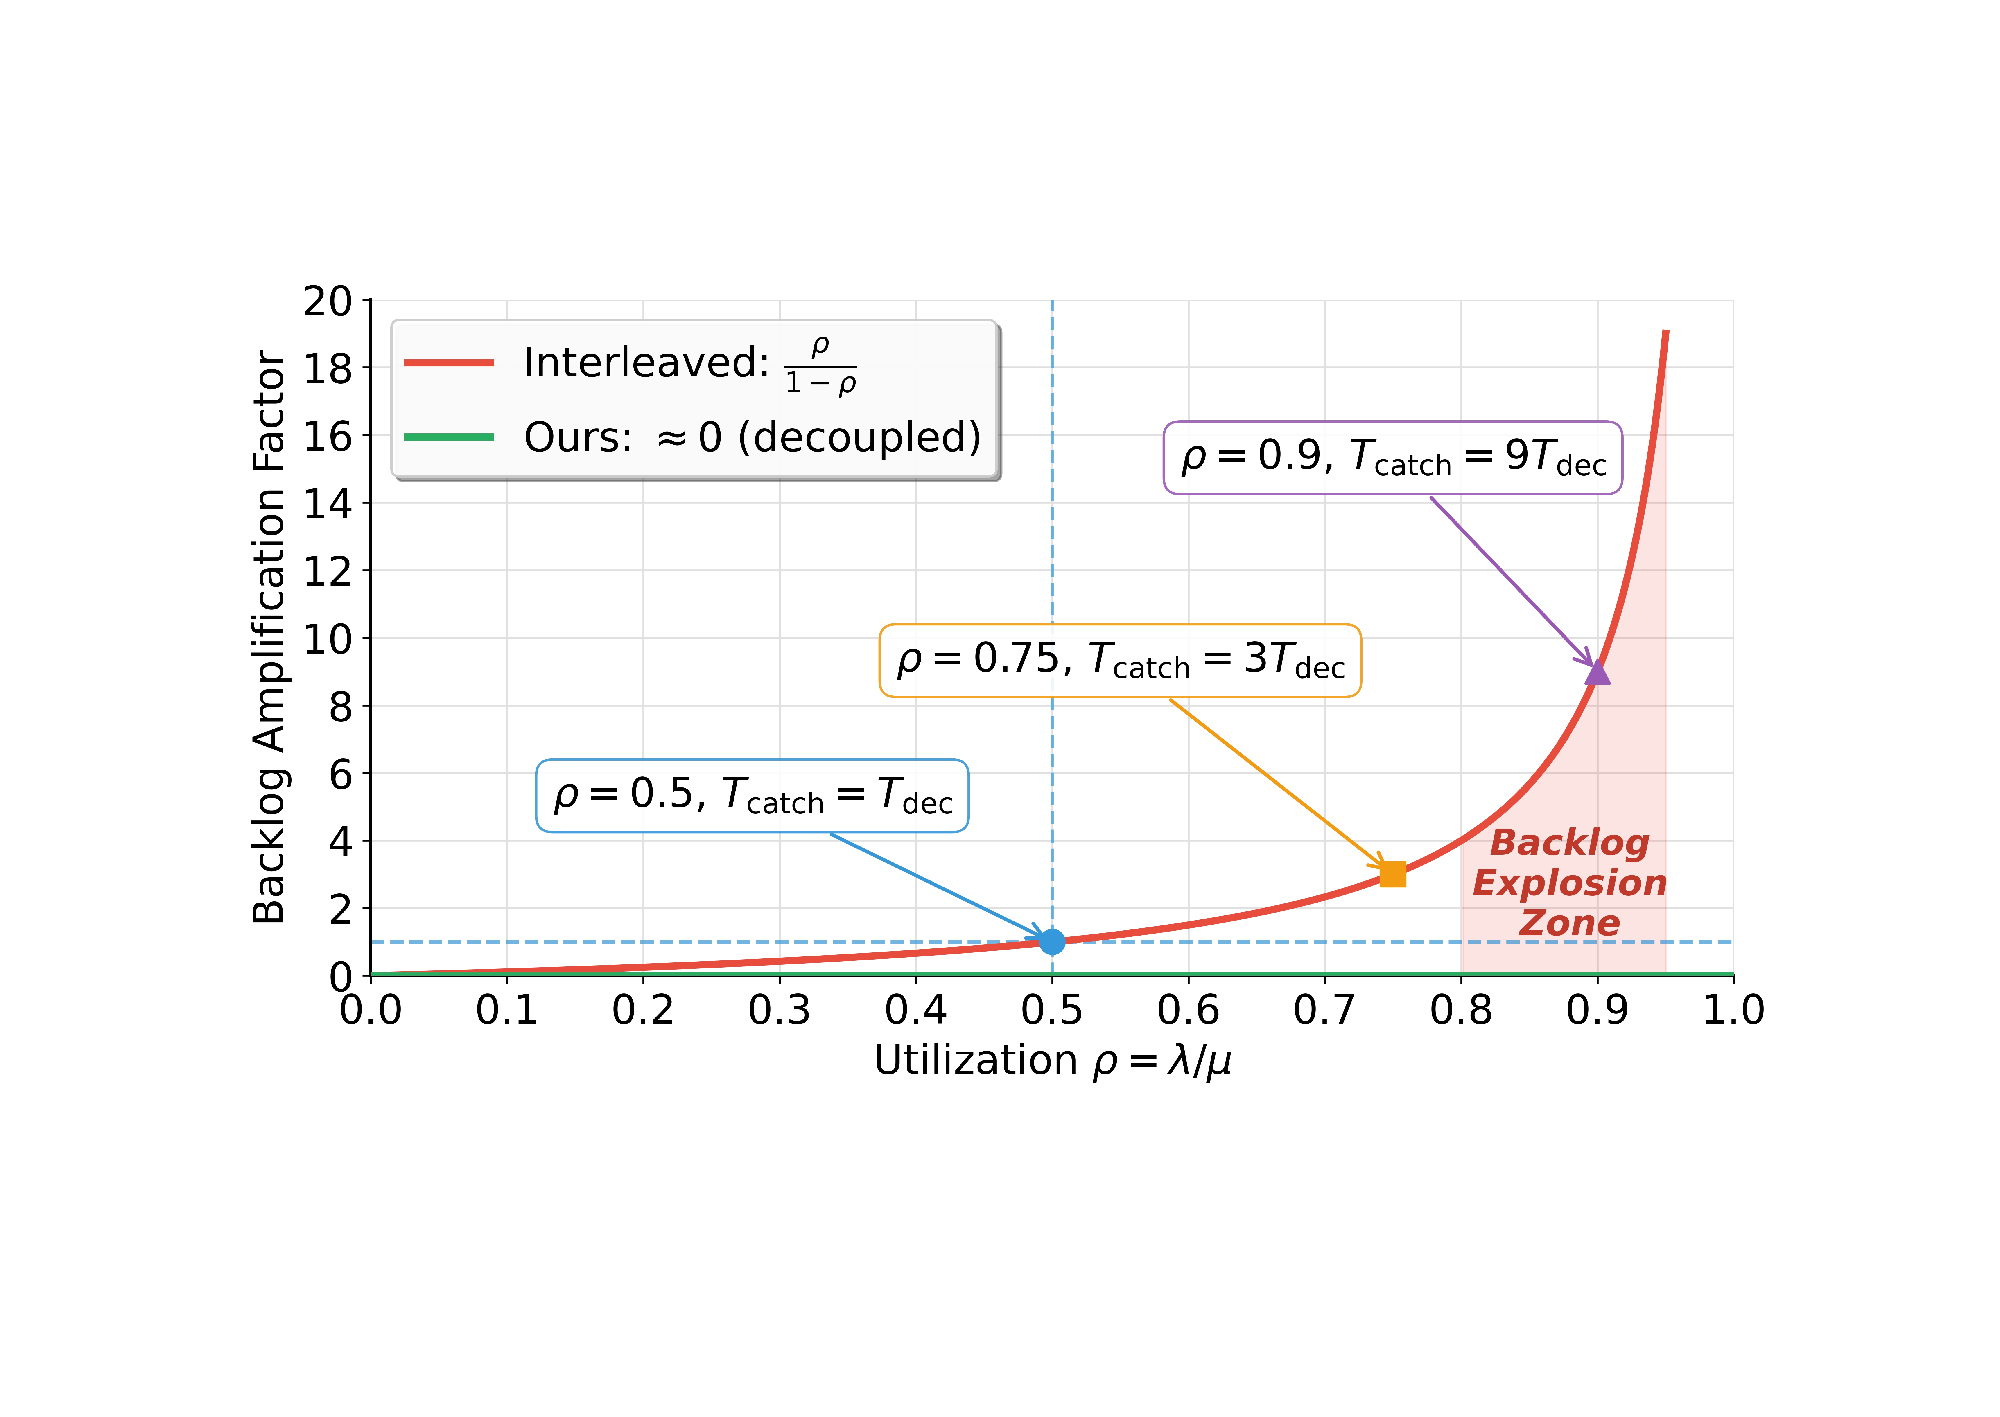
\includegraphics[width=0.72\linewidth]{Figure/latency.pdf}
  \caption{\textbf{Decoder-induced ingestion backlog under interleaved streaming.}
    As utilization $\rho$ increases, interleaved decoding pauses can amplify the catch-up delay and enter a backlog explosion regime, while our decoupled design substantially reduces decoder-induced backlog growth.}
  \label{fig:latency}
\end{figure}

\section{Additional Baseline Details}
\label{app:baselines}

\noindent\textbf{Flash-VStream-7B\cite{DBLP:journals/corr/abs-2506-23825}.}
Flash-VStream is an efficient video language model for long video streams. It introduces a flash memory module composed of a low-capacity context memory for aggregating long-range temporal information and a high-capacity augmentation memory for retrieving detailed spatial evidence, enabling real-time responses to user queries over extremely long videos.

\noindent\textbf{VideoLLM-online-8B\cite{DBLP:conf/cvpr/ChenLWLSGLGMS24}.}
VideoLLM-online proposes the LIVE framework, short for learning in video streams, to enable temporally aligned, long-context, and real-time conversation over continuous video streams. Specifically, LIVE introduces a streaming training objective, a data generation scheme that converts offline temporal annotations into streaming dialogue data, and an optimized inference pipeline with a continuous KV cache as well as parallelized visual encoding and language decoding for efficient online responses.

\noindent\textbf{Dispider-7B\cite{DBLP:conf/cvpr/0001DD0ZCL025}.}
Dispider targets active real-time interaction by explicitly disentangling perception, decision, and reaction. It uses a lightweight proactive streaming video processing module to continuously monitor the stream and identify suitable moments for interaction, while an asynchronous interaction module generates detailed responses without blocking continued observation.

\noindent\textbf{StreamForest-7B\cite{DBLP:journals/corr/abs-2509-24871}.}
StreamForest is designed for efficient online video understanding with persistent event memory. Its core Persistent Event Memory Forest organizes historical frames into event-level tree structures for long-term retention under limited computational resources, while a Fine-grained Spatiotemporal Window preserves detailed short-term perception.

\noindent\textbf{StreamAgent-7B\cite{DBLP:journals/corr/abs-2508-01875}.}
StreamAgent studies anticipatory agents for streaming video understanding. Instead of reacting only to current observations, it integrates question semantics and historical observations to anticipate future task-relevant temporal intervals and spatial regions, and combines this strategy with a streaming KV cache memory for selective recall, enabling proactive and goal-directed responses in evolving video streams.

\section{Dataset and Benchmark Details}
\label{app:data}

\subsection{Benchmark Details}
\label{app:benchmark-details}

\noindent\textbf{StreamingBench~\cite{lin2024streamingbenchassessinggapmllms}.}
StreamingBench is a benchmark tailored for streaming video understanding, containing 18 tasks over 900 videos and 4,500 human-curated QA pairs, where each question is associated with a specific timestamp in the video stream. The benchmark covers three major aspects of streaming understanding: real-time visual understanding, omnisource understanding, and contextual understanding. In our main tables, we further summarize the reported results into four subset-level metrics: \textbf{Realtime}, \textbf{OmniSource}, \textbf{SQA}, and \textbf{Proactive}. For evaluation, we follow the adaptive frame extraction protocol reported in StreamingBench: videos shorter than 5 minutes are sampled at 1 fps, videos between 5 and 10 minutes at 0.5 fps, and videos longer than 10 minutes at 0.2 fps.

\noindent\textbf{OVO-Bench~\cite{DBLP:conf/cvpr/NiuLMGZHDDD0ZZC25}.}
OVO-Bench is designed to evaluate online video understanding with explicit temporal awareness. It organizes evaluation into three subsets: \textbf{Backward}, which requires tracing back to past events; \textbf{Realtime}, which focuses on understanding what is happening at the current timestamp; and \textbf{Forward}, which evaluates whether the model can defer its response until sufficient future evidence becomes available. In our experiments, we follow the common OVO-Bench comparison setting for offline video LLMs and cap the visual input at no more than 64 frames per query.

\noindent\textbf{Video-MME~\cite{DBLP:conf/cvpr/FuDLLRZWZSZCLLZ25}.}
Video-MME is a comprehensive offline video benchmark with 900 videos and 2,700 multiple-choice QA pairs, spanning 6 primary visual domains and 30 subfields, and reporting results on \textbf{Short}, \textbf{Medium}, and \textbf{Long} duration subsets. To adapt Video-MME to our streaming-style evaluation, we aggregate all QA pairs sharing the same video ID into a single example and convert each video into an ordered stream of temporal segments. The model receives these segments sequentially, and the associated questions are issued only after the full video stream has been observed. This preserves the original benchmark content while turning Video-MME into a suffix-query streaming protocol.

\noindent\textbf{LV-Bench~\cite{wang2025lvbenchextremelongvideo}.}
LV-Bench is an extreme long-video benchmark for evaluating long-range video understanding. It measures six core capabilities, namely \textbf{ER} (Entity Recognition), \textbf{EU} (Event Understanding), \textbf{KIR} (Key Information Retrieval), \textbf{TG} (Temporal Grounding), \textbf{Rea} (Reasoning), and \textbf{Sum} (Summarization). In our adaptation, we first aggregate samples by video ID, and then use the end time of the official annotated time span as the segment boundary to construct a streaming input sequence. The model is queried when the stream reaches the corresponding boundary, making the evaluation compatible with our streaming inference pipeline while preserving the original supervision structure.

\begin{figure*}[t]
  \centering
  \begin{minipage}[t]{0.32\textwidth}
    \centering
    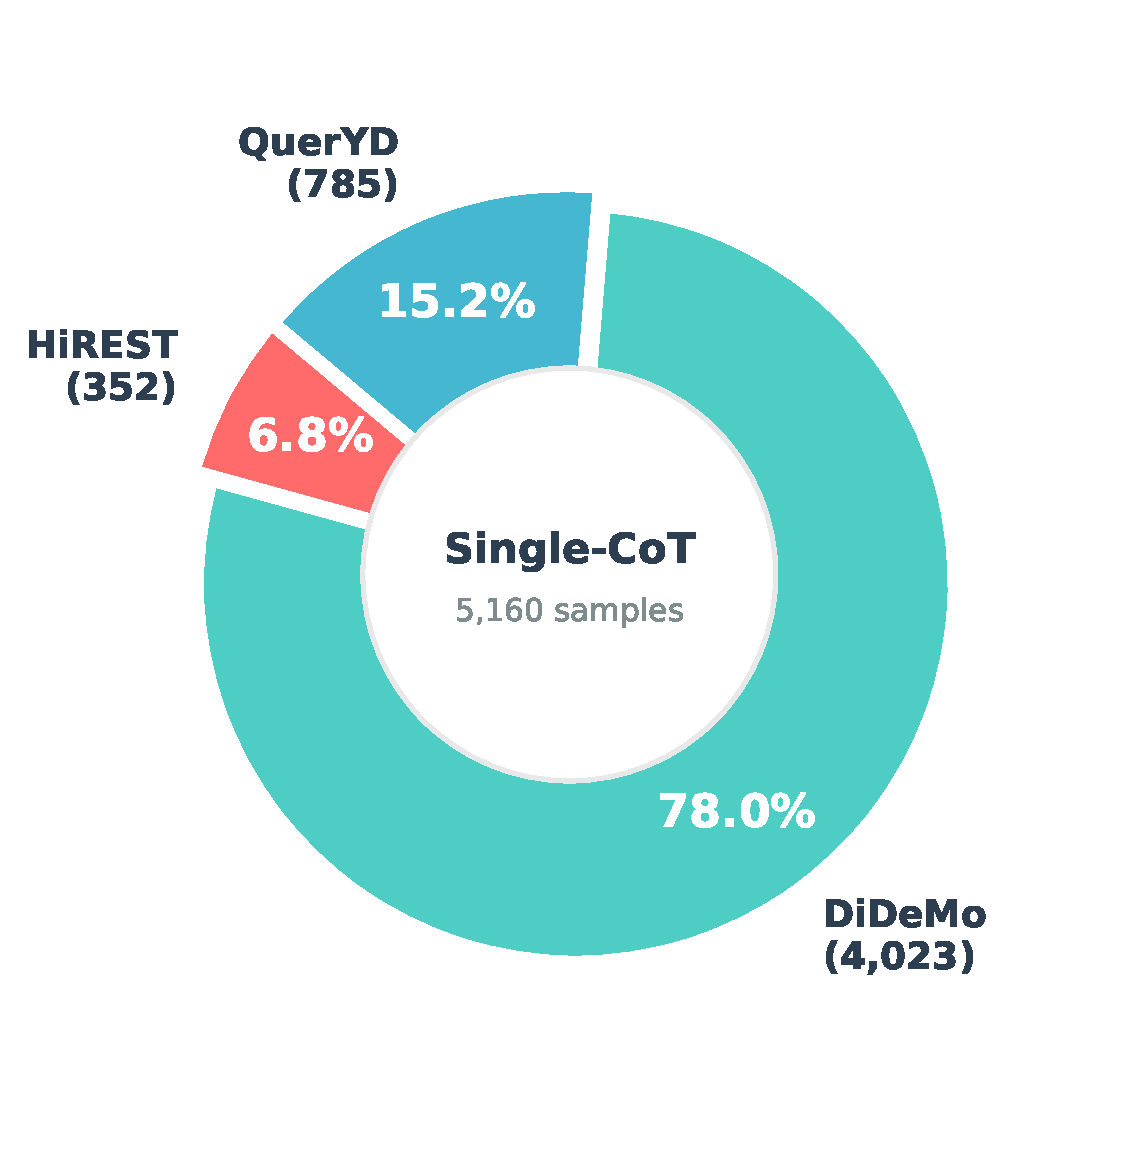
\includegraphics[width=\linewidth]{Figure/Appendix/single_cot_distribution.pdf}
    \par\small (a) Single-round CoT.
  \end{minipage}\hfill
  \begin{minipage}[t]{0.32\textwidth}
    \centering
    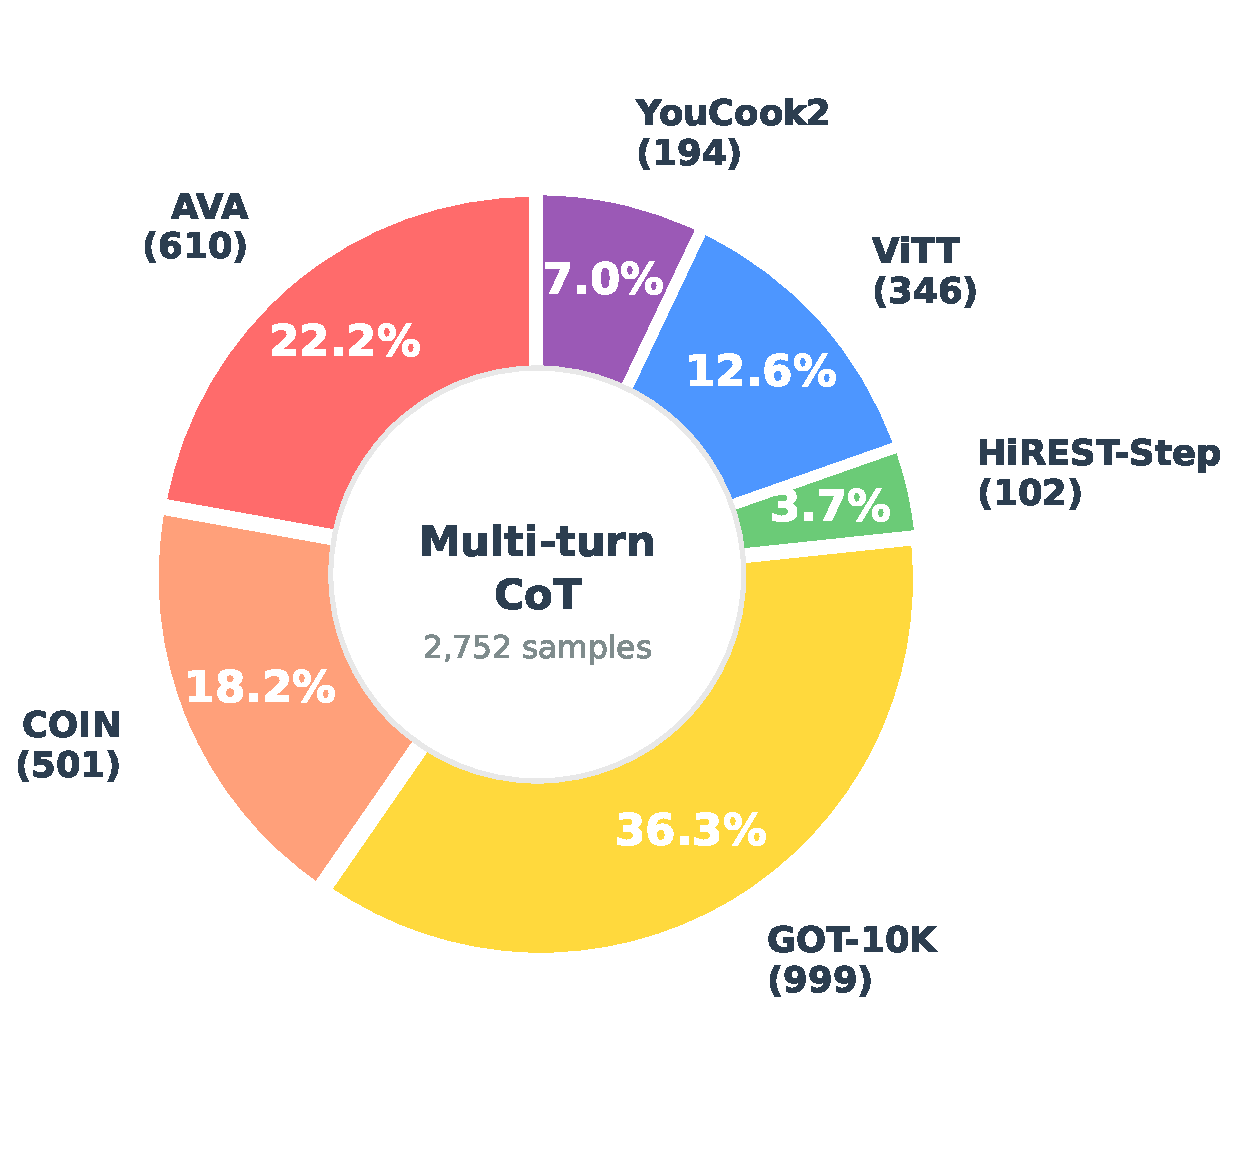
\includegraphics[width=\linewidth]{Figure/Appendix/multi_turn_cot_distribution.pdf}
    \par\small (b) Multi-round CoT.
  \end{minipage}\hfill
  \begin{minipage}[t]{0.32\textwidth}
    \centering
    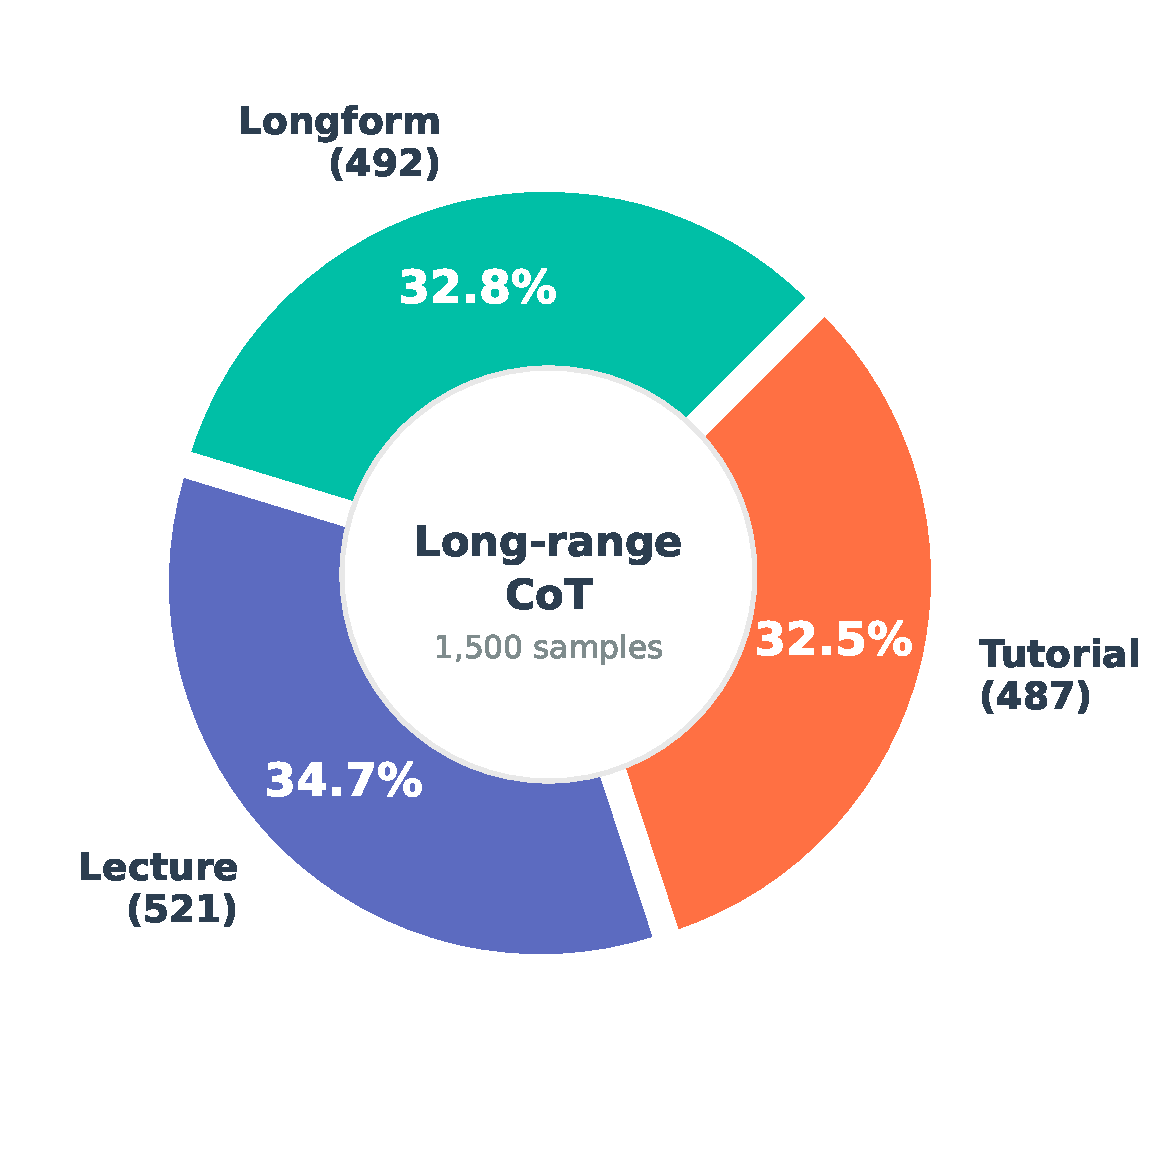
\includegraphics[width=\linewidth]{Figure/Appendix/long_range_cot_distribution.pdf}
    \par\small (c) Long-range CoT.
  \end{minipage}
  \caption{\textbf{Dataset composition}}
  \label{fig:data-distributions}
\end{figure*}

\subsection{Overall Dataset Composition}
\label{app:data-composition}

Figure~\ref{fig:data-distributions} visualizes the three-stage data composition and its alignment with our training objectives: Stage~1 for single-round memory writing and answering, Stage~2 for multi-round consistency, and Stage~3 for long-horizon recall, uncertainty handling, and distractor robustness.

\noindent\textbf{VideoChatOnline-IT Source Pool.}
Stage~1 and Stage~2 are both constructed from VideoChatOnline-IT, a video instruction-tuning corpus for online video understanding. It unifies multiple temporally grounded video QA sources in a streaming-style format, making it a suitable source pool for our pseudo streaming chain-of-thought (CoT) construction. We use different subsets for different training objectives. Stage~1 targets single-round streaming CoT and uses HiREST, DiDeMo, and QuerYD. Stage~2 targets multi-round streaming CoT and uses AVA, COIN, GOT-10K, HiREST-Step, ViTT, and YouCook2. Detailed statistics are reported in Table~\ref{tab:single-cot} and Table~\ref{tab:multi-turn-detail}.

\noindent\textbf{Stage 1: Single-round CoT Statistics.}
\label{app:single-cot}
Stage~1 focuses on training the model to write segment-level memory notes and answer a single streaming question grounded in the observed prefix. Table~\ref{tab:single-cot} reports the breakdown by source subset.

\begin{table}[!htbp]
  \caption{\textbf{Stage 1 detailed statistics.}}
  \label{tab:single-cot}
  \centering
  \small
  \begin{tabular}{lrr}
    \toprule
    \textbf{Subset} & \textbf{Samples} & \textbf{Proportion (\%)} \\
    \midrule
    HiREST & 352 & 6.8 \\
    DiDeMo & 4023 & 78.0 \\
    QuerYD & 785 & 15.2 \\
    \midrule
    Total & 5,160 & 100.0 \\
    \bottomrule
  \end{tabular}
\end{table}

\noindent\textbf{Stage 2: Multi-round CoT Statistics.}
\label{app:multi-turn-cot}
Stage~2 trains multi-turn consistency: later answers must reuse earlier segment-level memory notes without peeking into future segments. Table~\ref{tab:multi-turn-detail} reports detailed statistics, including the number of segments and questions aggregated from the underlying sources.

\begin{table}[!htbp]
  \caption{\textbf{Stage 2 detailed statistics.}
  Segments counts the number of segment units after stream segmentation, and Questions counts the number of question turns in the synthesized dialogues. Avg. Segs. and Avg. Qs. denote the average numbers of segments and questions per sample.}
  \label{tab:multi-turn-detail}
  \centering
  \small
  \begin{tabular}{lrrrrr}
    \toprule
    \textbf{Subset} & \textbf{Samples} & \textbf{Segments} & \textbf{Questions} & \textbf{Avg. Segs.} & \textbf{Avg. Qs} \\
    \midrule
    AVA & 610 & 6,136 & 1,902 & 10.06 & 3.12 \\
    COIN & 501 & 2,793 & 1,109 & 5.57 & 2.21 \\
    GOT-10K & 999 & 2,830 & 2,820 & 2.83 & 2.82 \\
    HiREST-Step & 102 & 320 & 422 & 3.14 & 4.14 \\
    ViTT & 346 & 1,090 & 1,436 & 3.15 & 4.15 \\
    YouCook2 & 194 & 630 & 824 & 3.25 & 4.25 \\
    \midrule
    Total & 2,752 & 13,799 & 8,513 & 5.01 & 3.09 \\
    \bottomrule
  \end{tabular}
\end{table}

\noindent\textbf{Stage 3: Long-range CoT Statistics and Retrieval Keywords.}
\label{app:stage3}
Stage~3 targets long-horizon streaming behaviors on long videos collected from YouTube. We use 500+ keywords to retrieve candidate long videos, covering procedural workflows (tutorial), explanatory content (lecture), and continuous recordings (longform). Table~\ref{tab:stage3-detail} reports the resulting dataset statistics by category, and Table~\ref{tab:yt-queries} lists representative query examples used for video retrieval.

\begin{table}[t]
  \caption{\textbf{Stage 3 statistics by category.}}
  \label{tab:stage3-detail}
  \centering
  \small
  \begin{tabular}{lrrrrr}
    \toprule
    \textbf{Category} & \textbf{Samples} & \textbf{Segments} & \textbf{Questions} & \textbf{Avg. Segs.} & \textbf{Avg. Qs} \\
    \midrule
    Tutorial & 487 & 5,631 & 2,017 & 11.56 & 4.14 \\
    Lecture  & 521 & 4,532 & 1,893 & 8.70  & 3.63 \\
    Longform & 492 & 5,536 & 2,090 & 11.25 & 4.25 \\
    \midrule
    Total & 1,500 & 15,699 & 6,000 & 10.47 & 4.00 \\
    \bottomrule
  \end{tabular}
\end{table}

\begin{table}[H]
\caption{\textbf{Core constraints for pseudo streaming CoT generation.}}
\label{tab:prompt-constraints}
\centering
\small
\begin{tabular}{p{0.08\textwidth}p{0.84\textwidth}}
\toprule
\textbf{ID} & \textbf{Constraint} \\
\midrule
A & \textbf{Strict one-to-one alignment:} exactly one output chunk per input unit, preserving order. \\
B & \textbf{No empty segment:} each segment must update/maintain grounded state based on visual evidence. \\
C & \textbf{No future information:} segment reasoning uses only current and past units; QA uses evidence up to its timestamp. \\
D & \textbf{No answer leakage:} do not reveal reference answers in reasoning; copy the answer only in the final Answer field. \\
E & \textbf{Video-grounded only:} rely on provided frames/timestamps/metadata; avoid external assumptions. \\
F & \textbf{Streaming quality:} emphasize boundary cues and conservative state updates across segments. \\
G & \textbf{Question awareness:} track unanswered questions and prioritize collecting relevant evidence online. \\
\bottomrule
\end{tabular}
\end{table}

\begin{table}[t]
  \caption{\textbf{Representative YouTube search queries used for Stage~3 video retrieval.}}
  \label{tab:yt-queries}
  \centering
  \small
  \setlength{\tabcolsep}{4pt}
  \renewcommand{\arraystretch}{1.05}
  \begin{tabular}{p{0.44\textwidth}p{0.42\textwidth}}
    \toprule
    \textbf{Query keyword} & \textbf{Video type} \\
    \midrule
    \multicolumn{2}{l}{\textbf{Tutorial}} \\
    \texttt{sourdough bread tutorial} & Complete bread-making workflow \\
    \texttt{furniture restoration} & Furniture restoration project \\
    \texttt{oil painting tutorial} & Oil painting step-by-step tutorial \\
    \texttt{car repair tutorial complete} & Full car repair walkthrough \\
    \texttt{sewing tutorial complete} & Complete sewing tutorial \\
    \texttt{woodworking project tutorial} & Woodworking project tutorial \\
    \texttt{pottery making tutorial} & Pottery making process \\
    \texttt{knife making tutorial} & Knife forging tutorial \\
    \addlinespace[0.3em]

    \multicolumn{2}{l}{\textbf{Lecture}} \\
    \texttt{machine learning lecture} & Machine learning course lecture \\
    \texttt{organic chemistry lecture} & Organic chemistry lecture \\
    \texttt{quantum mechanics lecture} & Quantum mechanics lecture \\
    \texttt{algorithm course full} & Full algorithm course \\
    \texttt{system design lecture} & System design lecture \\
    \texttt{neuroscience lecture} & Neuroscience lecture \\
    \texttt{deep learning tutorial} & Deep learning lecture/tutorial \\
    \texttt{computer vision lecture} & Computer vision lecture \\
    \addlinespace[0.3em]

    \multicolumn{2}{l}{\textbf{Longform}} \\
    \texttt{hiking trail complete} & Full hiking trail recording \\
    \texttt{train journey scenic} & Scenic train journey \\
    \texttt{safari wildlife documentary} & Safari wildlife documentary \\
    \texttt{Tokyo walking tour} & City walking tour (Tokyo) \\
    \texttt{northern lights footage} & Northern lights raw footage \\
    \texttt{coral reef documentary} & Coral reef documentary \\
    \texttt{mountain climbing documentary} & Mountain climbing documentary \\
    \texttt{storm chasing footage} & Storm chasing raw footage \\
    \bottomrule
  \end{tabular}
\end{table}

\subsection{Pseudo Streaming CoT Generation Principles}
\label{app:synthesis-principles}

We synthesize pseudo streaming CoT annotations to match the streaming protocol in Sec.~\ref{sec:paradigm}. A key constraint is strict alignment: for a stream with $S$ segments and $Q$ questions, the synthesized output must contain exactly $S+Q$ generated items, one for each interleaved unit and in temporal order. Table~\ref{tab:prompt-constraints} summarizes the core constraints enforced during CoT synthesis.

\noindent\textbf{Prompt template.}
For reproducibility, we provide the complete prompt used to synthesize pseudo streaming CoT. We use special tokens to delimit streaming units: \texttt{$<$EOS$>$} ends an input segment unit, \texttt{$<$EOQ$>$} ends an input question unit (and also the corresponding QA output), and \texttt{$<$EOT$>$} ends a generated segment-reasoning chunk. In training data, we keep only essential delimiters to reduce overfitting to superficial formatting.

\begin{PromptBox}
general_prompt = '''
You are a pseudo streaming Video Chain-of-Thought (CoT) generator.
You will receive the FULL input at once (all video segments + all questions + reference answers),
but you MUST generate reasoning that looks as if you processed the video incrementally, in time order.
====================
1) CORE CONSTRAINTS
====================
(A) STRICT ONE-TO-ONE ALIGNMENT (mandatory)
- The input is a chronological sequence of interleaved units.
- Video segment units end with <EOS>.
- Question units end with <EOQ>.
- You MUST output exactly ONE reasoning chunk per input unit.
- Output order must exactly match input order.
- Total output chunks = (#segment units + #question units).
- Do NOT merge units.
- Do NOT split units.
- Do NOT reorder units.
(B) EVERY SEGMENT REQUIRES REASONING (no empty segments)
- For every video segment unit, produce meaningful reasoning grounded in that segment.
- If no task-relevant change occurs, explicitly state that the scene, action, or tracked state remains stable.
- Avoid meta statements; focus on video evidence and state continuity.
(C) pseudo streaming / NO FUTURE INFORMATION
- Although you see the full input, behave as if you only know information up to the current unit.
- In [SEG k THINK], you may ONLY use evidence from segment k and all earlier segments.
- NEVER use or hint at information that appears only in future segments, questions, or answers.
- In [Q j THINK], reason ONLY with evidence available up to the question timestamp t.
(D) NO ANSWER LEAKAGE
- Each question includes a Reference Answer (for alignment only).
- NEVER reveal, paraphrase, or hint at any reference answer in any segment reasoning.
- In [Q j THINK], output the final answer ONLY inside the Answer field.
- The Answer MUST be copied EXACTLY and VERBATIM from the Reference Answer.
- Do NOT leak the answer in the Reasoning field.
(E) VIDEO-GROUNDED ONLY
- Use only visual evidence provided by frames, timestamps, bounding boxes, and metadata.
- Do NOT rely on external knowledge, assumptions, or commonsense completion.
(F) STREAMING VIDEO REASONING QUALITY
Each segment reasoning should:
- Describe what is visually observed or confirmed in this segment.
- Emphasize continuity, change, or boundary cues (start / end / ongoing).
- Update internal task-specific state clearly and conservatively.
(G) QUESTION AWARENESS (when applicable)
- If one or more questions have appeared:
  - Maintain an "Active Question": the earliest question that has not been answered.
  - Segment reasoning should prioritize collecting evidence relevant to the Active Question.
- If NO question has appeared yet:
  - Focus ONLY on understanding the video stream itself: scene setup, object/person continuity,
    motion patterns, emerging actions.
  - Do NOT speculate about future questions.
====================
2) INPUT FORMAT
====================
Units are interleaved in chronological order.
Video segment unit:
[SEG k | time = start-end | frames = ... | optional: bboxes / ids / actions] <EOS>
Question unit:
[Q j | t = timestamp]
Question: ...
Reference Answer: ...
<EOQ>
Notes:
- Timestamps may not start at 0; follow the provided time system exactly.
- Reference Answers are provided for alignment only.
====================
3) OUTPUT FORMAT (STRICT)
====================
For each video segment unit:
[SEG k THINK]
Focus: (either the Active Question in <= 15 words, OR "video understanding (no question yet)")
Evidence from this segment: (2-5 sentences, strictly video-grounded)
State update: (1-3 sentences, task-specific state or continuity)
<EOT>

For each question unit:
[Q j THINK]
Reasoning: (2-6 sentences, justify the answer using ONLY evidence available up to time t;
           you may reference segment indices/timestamps, but MUST NOT use future units
           and MUST NOT reveal/paraphrase the Reference Answer in Reasoning)
Answer: (copy the Reference Answer EXACTLY and VERBATIM)
<EOQ>
'''
\end{PromptBox}

\section{Case Studies}
\label{app:Study_Case}

This section presents three qualitative examples that complement the quantitative results. \Cref{fig:qual-single} shows a dataset-derived pseudo streaming CoT example under the single-round protocol. \Cref{fig:qual-multi} shows a dataset-derived pseudo streaming CoT example under the multi-round protocol. \Cref{fig:qual-case-study} shows a real multi-round streaming example and illustrates how segment-level memory supports cross-turn reference resolution and temporal state tracking.

\section{Error Analysis}
\label{app:error}

Although Stage~3 substantially improves long-horizon streaming reasoning, representative residual failures still remain in challenging multi-turn settings. Consistent with the three long-horizon behaviors explicitly targeted in Stage~3 training---long-term evidence retention, uncertainty handling, and distractor learning, as described in Sec.~\ref{sec:method:data}---we observe three recurring error patterns. First, the model may retain the coarse event trace while forgetting an early fine-grained attribute, such as which object, side, or entity was involved. This is consistent with our segment-level memory design: compact memory notes support long-range access but can still over-compress details over long temporal gaps. Second, under incomplete evidence, the model may commit to a specific hypothesis too early rather than deferring judgment until decisive visual evidence appears, reflecting a residual limitation of the uncertainty-handling objective in Sec.~\ref{sec:method:data}. Third, later retrieval can still be corrupted by visually salient but task-irrelevant segments, causing recent distractors to override the true earlier evidence. This aligns with the ablation results in Table~\ref{tab:memory_ablation}, which show that memory notes help stabilize retrieval but remain limited by the quality of written evidence and incoming visual context. As shown in Fig.~\ref{fig:error_cases}, these failures are residual edge cases of (a) long-range recall failure, (b) premature commitment under incomplete evidence, and (c) distractor-induced memory contamination in streaming multi-turn reasoning.

\begin{figure*}[p]
  \centering
  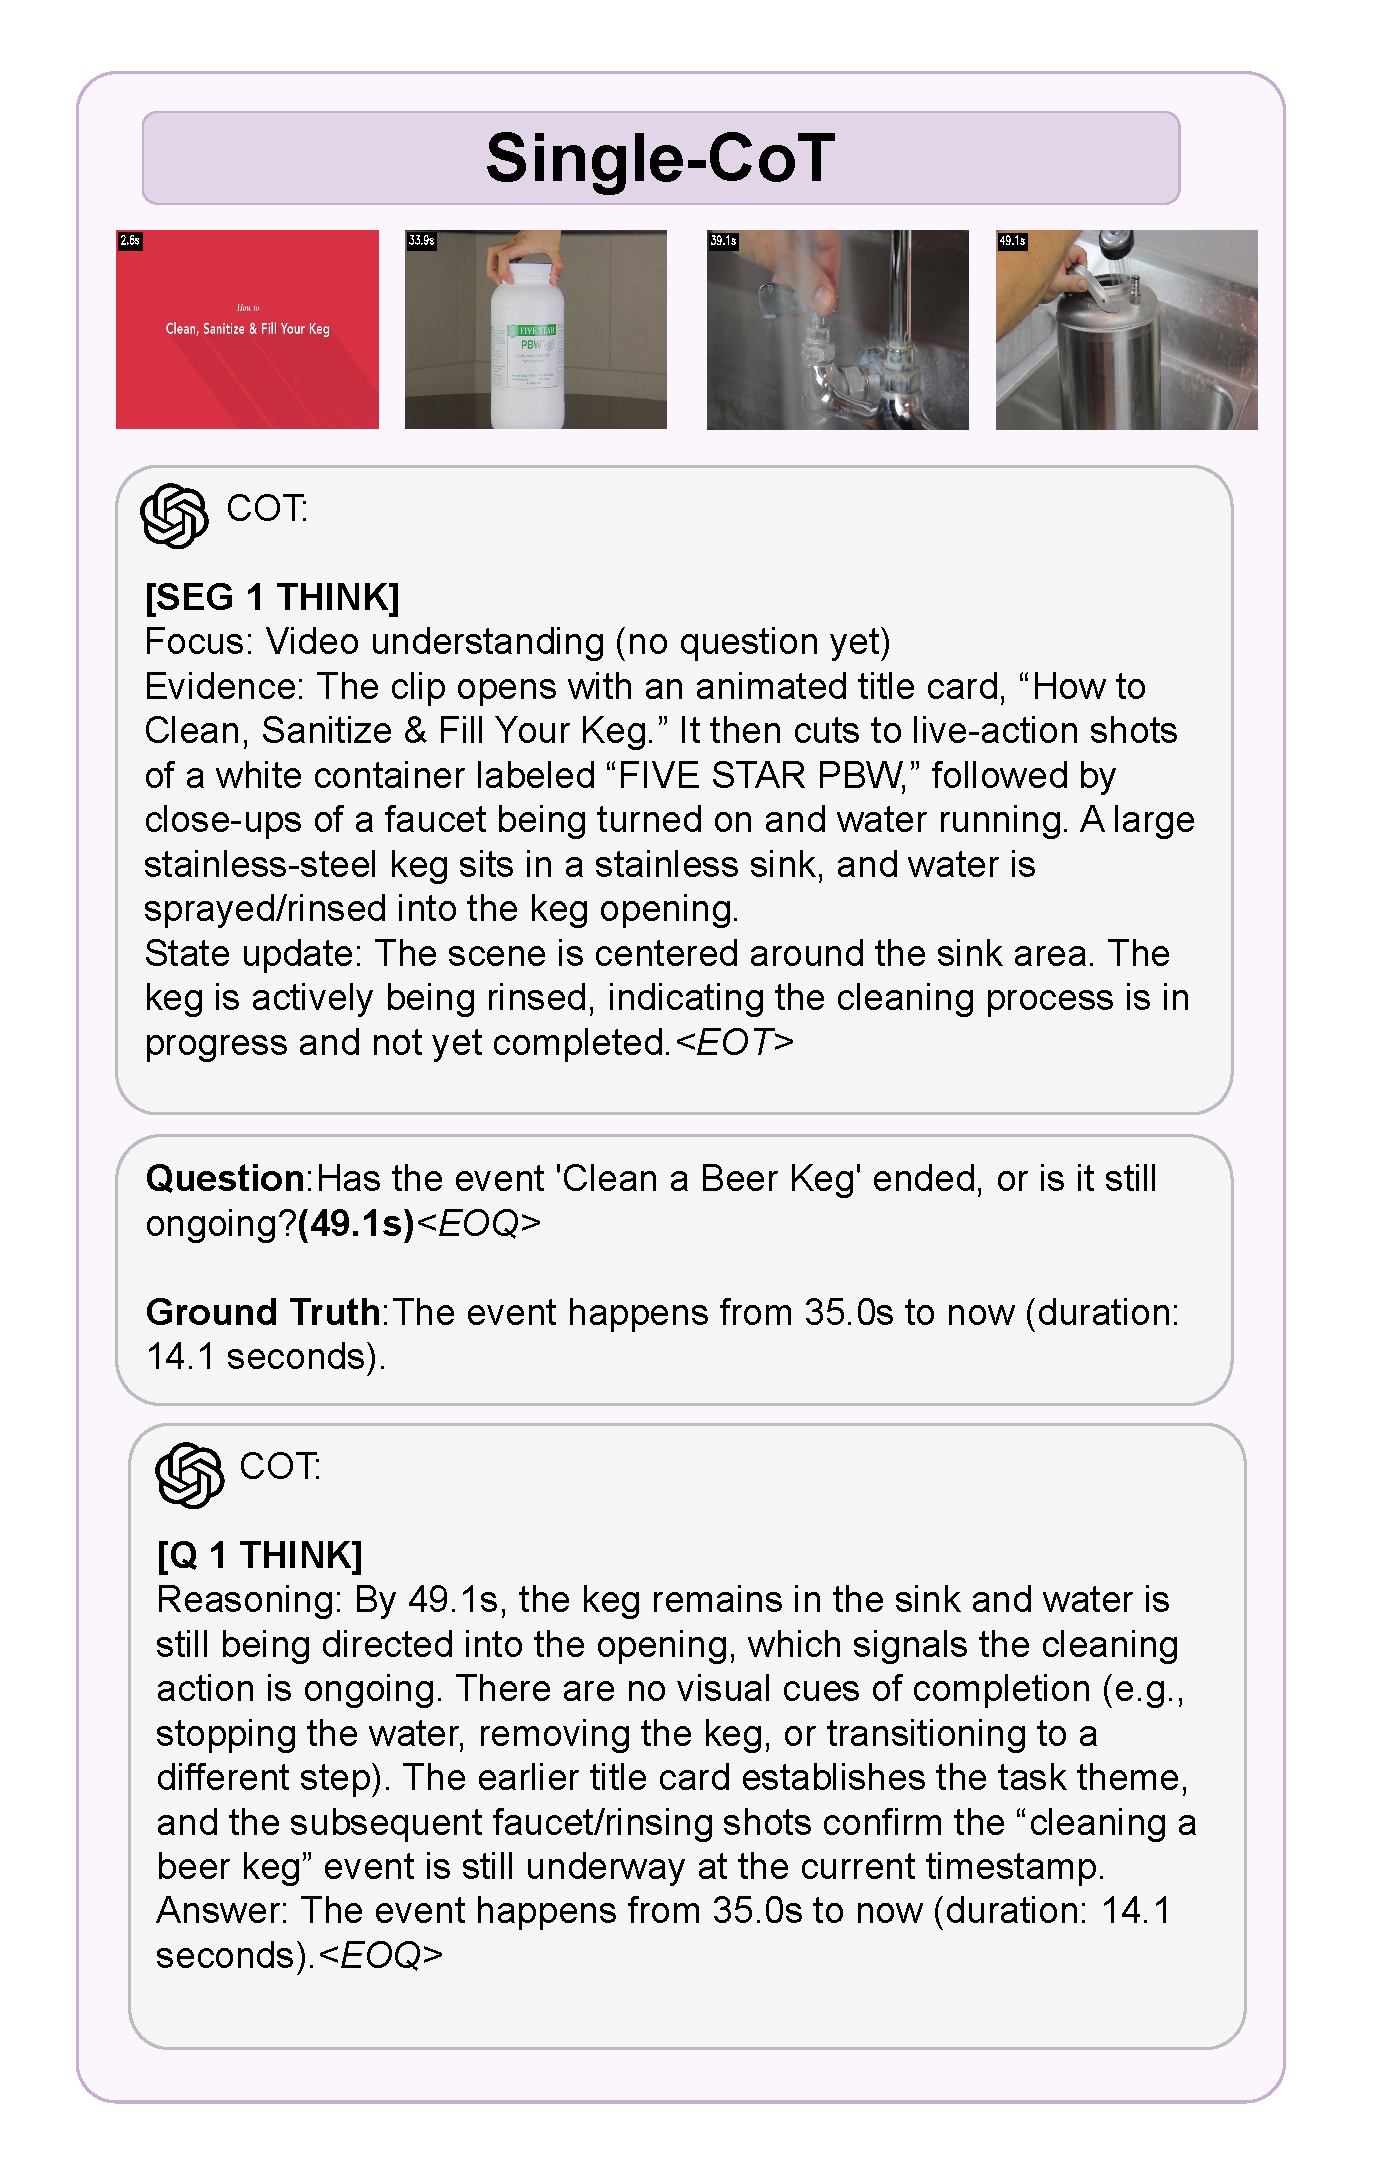
\includegraphics[width=\textwidth,height=0.85\textheight,keepaspectratio]{Figure/single.pdf}
  \caption{\textbf{Dataset-derived pseudo streaming CoT example under the single-round protocol.}
  A question is asked once after the observed video prefix. The model first writes a segment-level memory note from the incoming frames, identifying the tutorial title card, the cleaning material, the faucet, and the rinsing action around the keg. When queried at 49.1s, it answers using only the accumulated evidence so far and correctly concludes that the event \textbf{Clean a Beer Keg} is still ongoing.}
  \label{fig:qual-single}
\end{figure*}

\clearpage
\begin{figure*}[p]
  \centering
  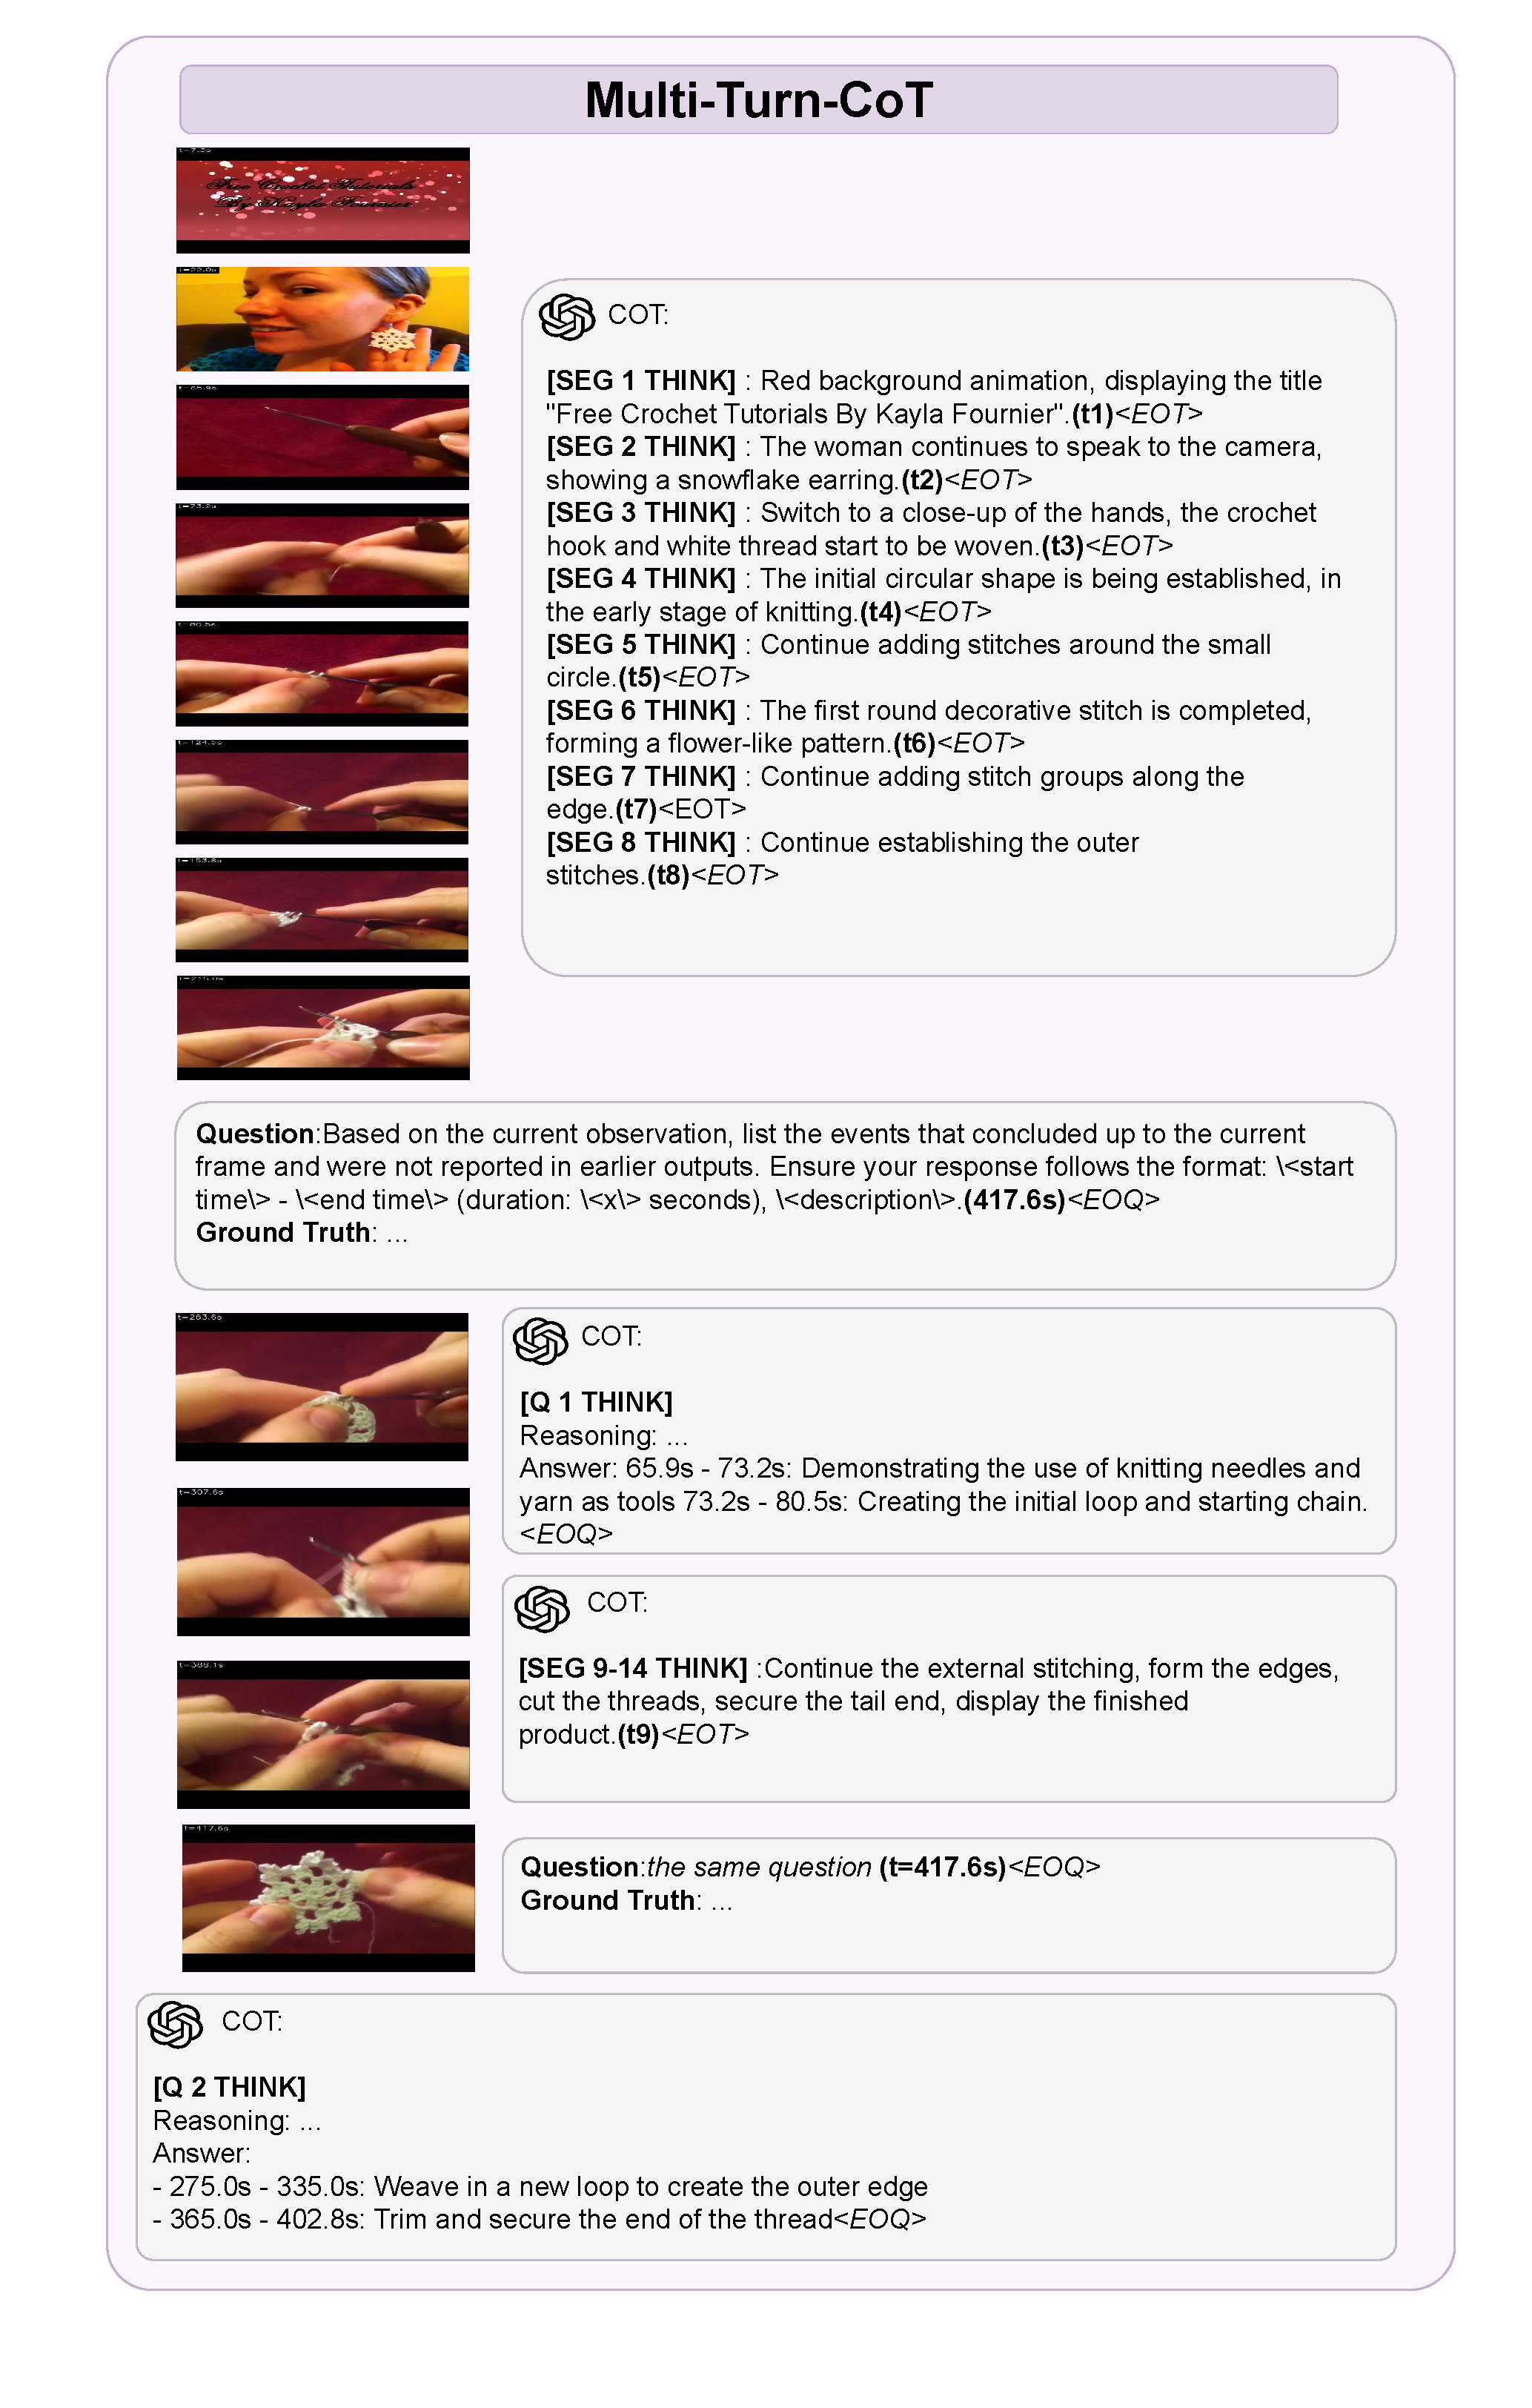
\includegraphics[width=\textwidth,height=0.85\textheight,keepaspectratio]{Figure/Multi-Turn.pdf}
  \caption{\textbf{Dataset-derived pseudo streaming CoT example under the multi-round protocol.}
 The stream follows a crochet tutorial. Memory notes from Segments 1 to 8 trace the progression from the introduction to close-up hand actions and the gradual formation of the crochet pattern. After the first event-listing question, the model reports only the completed events observed so far. As additional segments arrive, it updates the memory with later stitching and finishing steps. When the same question is asked again at 417.6s, the answer includes only the newly completed events that were not reported earlier, which illustrates incremental reasoning across multiple turns over a continuous stream.}
  \label{fig:qual-multi}
\end{figure*}

\clearpage
\begin{figure*}[p]
  \centering
  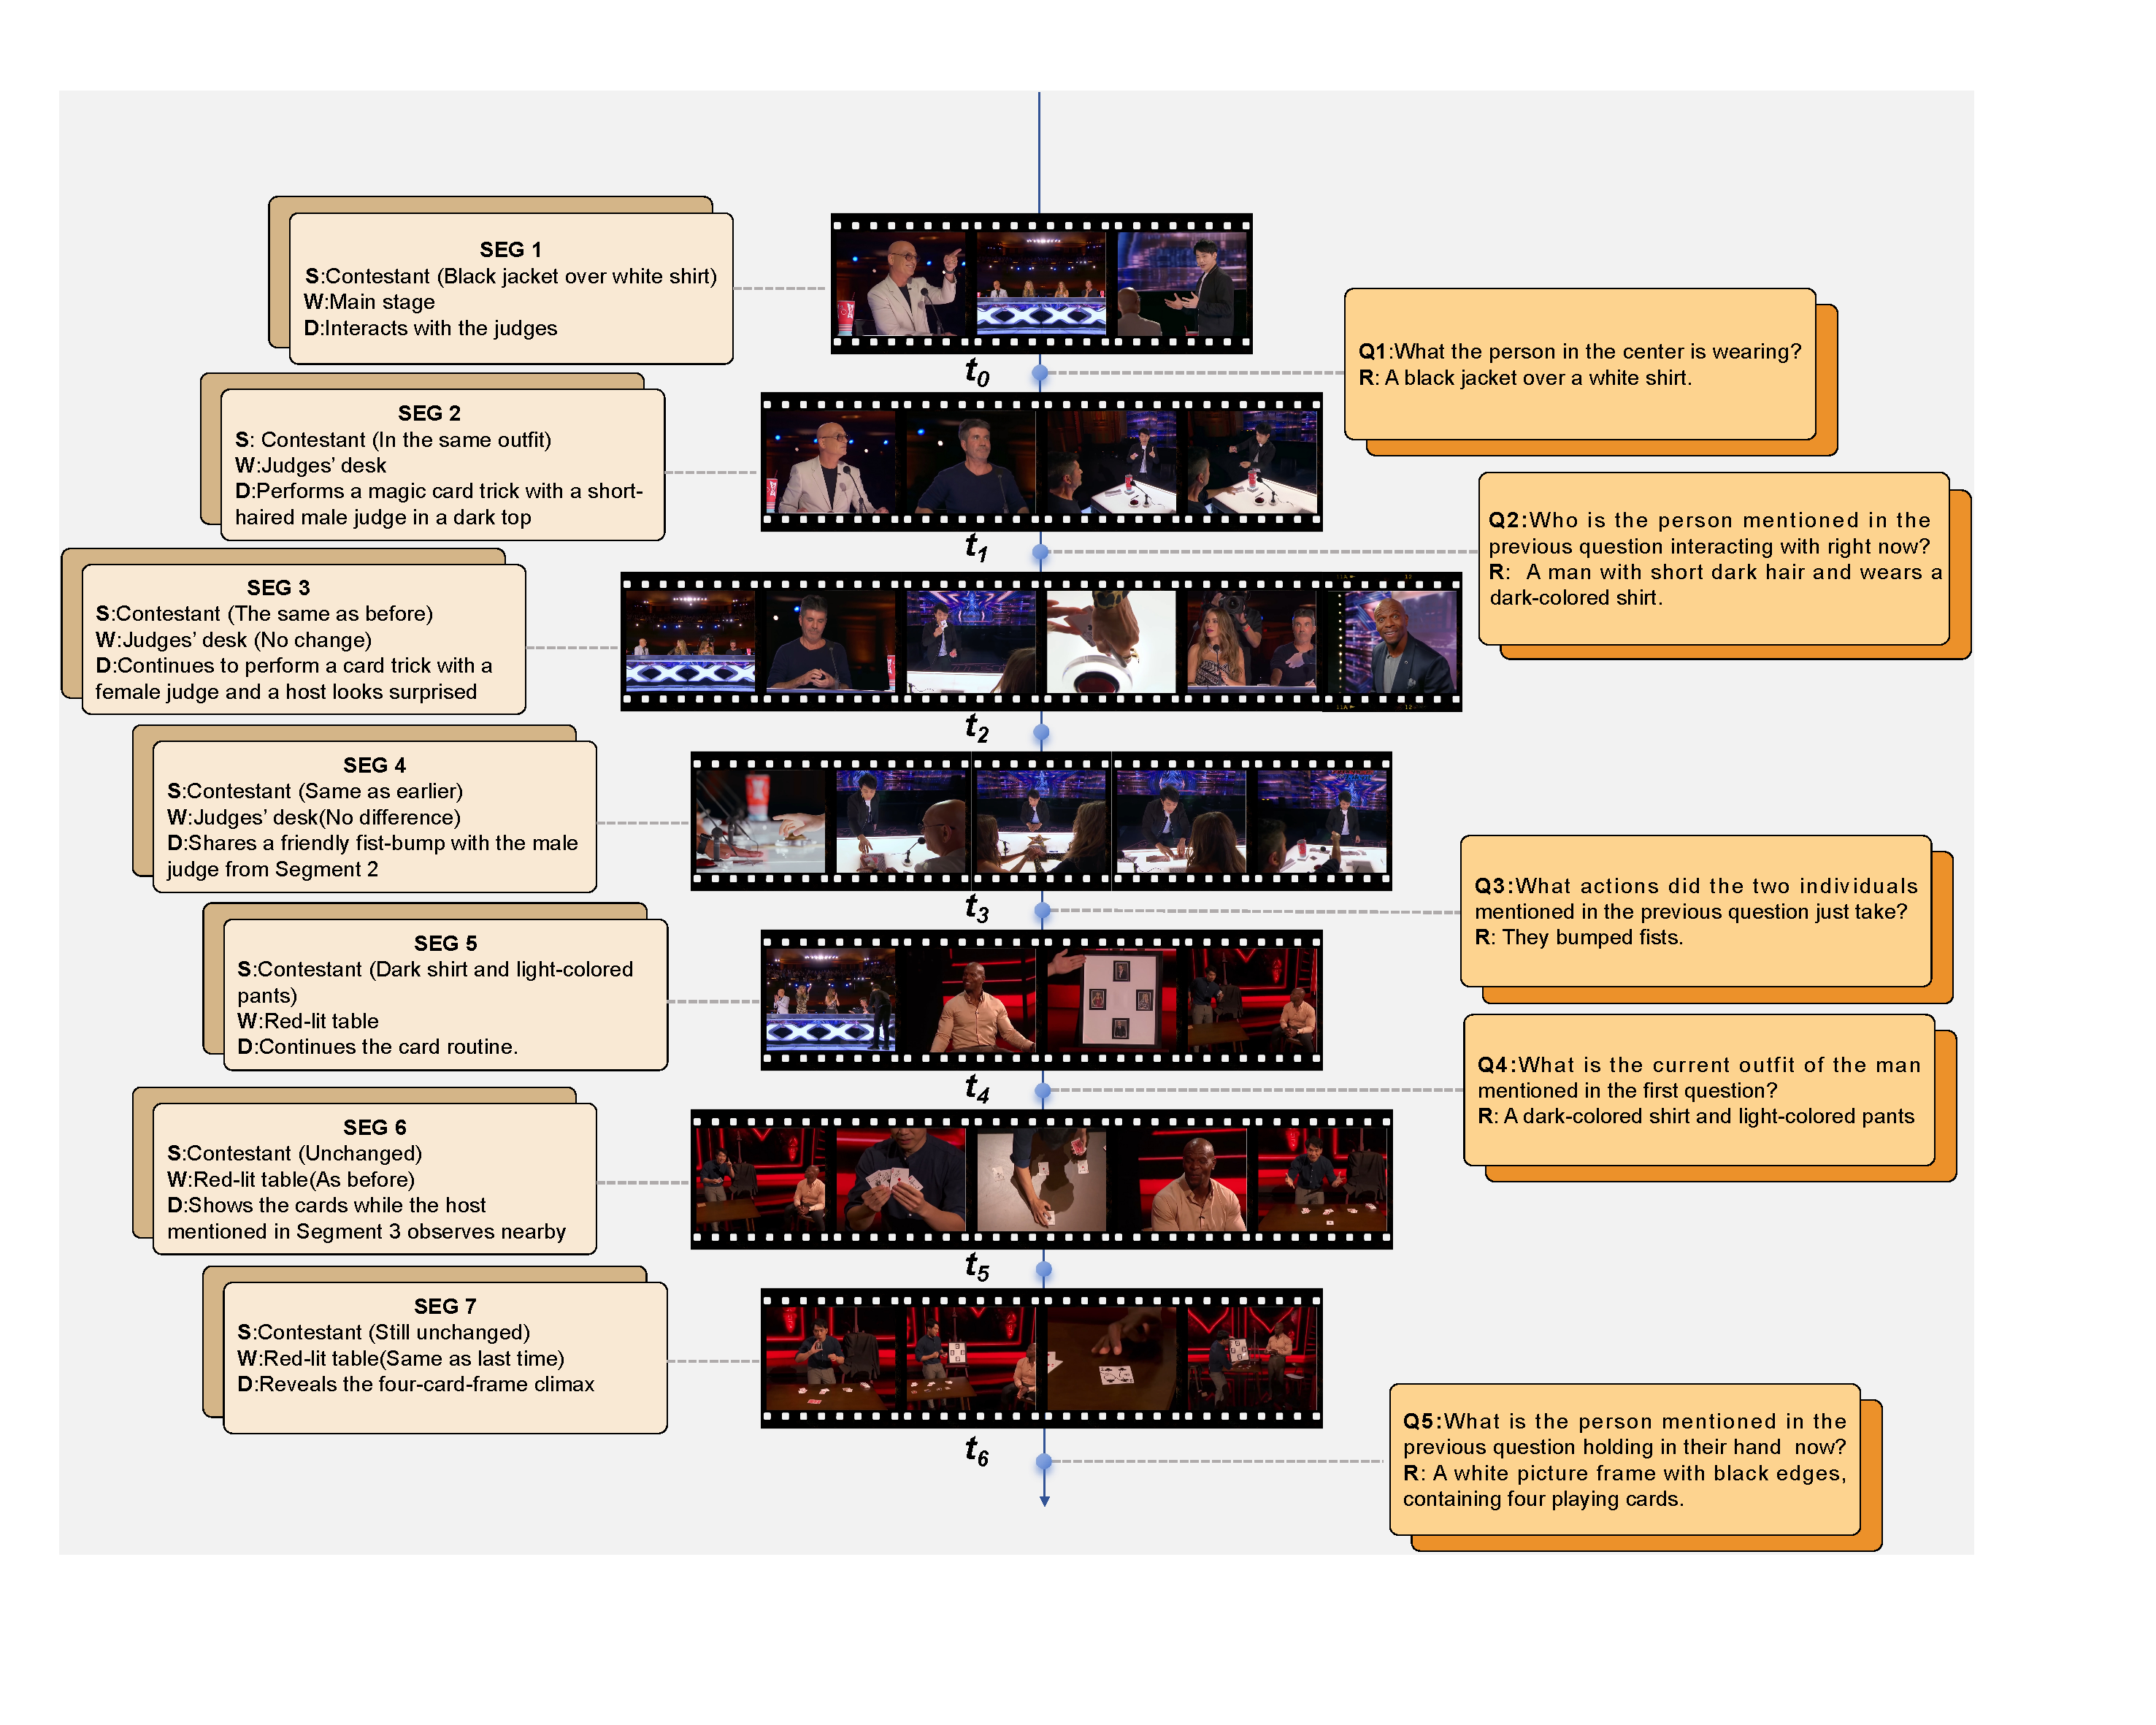
\includegraphics[width=\textwidth,height=0.80\textheight,keepaspectratio]{Figure/case_study.pdf}
  \caption{\textbf{Real multi-round streaming example.}
  Left: Segment-level memory notes summarize the contestant's appearance, location, and actions across seven streamed segments. Middle: Representative frames show the progression of a card routine from the main stage to the judges' desk and finally to a red-lit table. Right: Five temporally ordered questions are interleaved with the stream. Questions Q2 to Q5 depend on earlier turns, requiring the model to resolve the previously mentioned person, identify the current interaction partner, recall the recent fist bump, update the contestant's outfit after the scene transition, and track the object held in hand at the end. This example illustrates how persistent segment-level memory supports consistent reasoning across multiple turns over a changing stream.}
  \label{fig:qual-case-study}
\end{figure*}

\clearpage
\begin{figure*}[p]
  \centering
  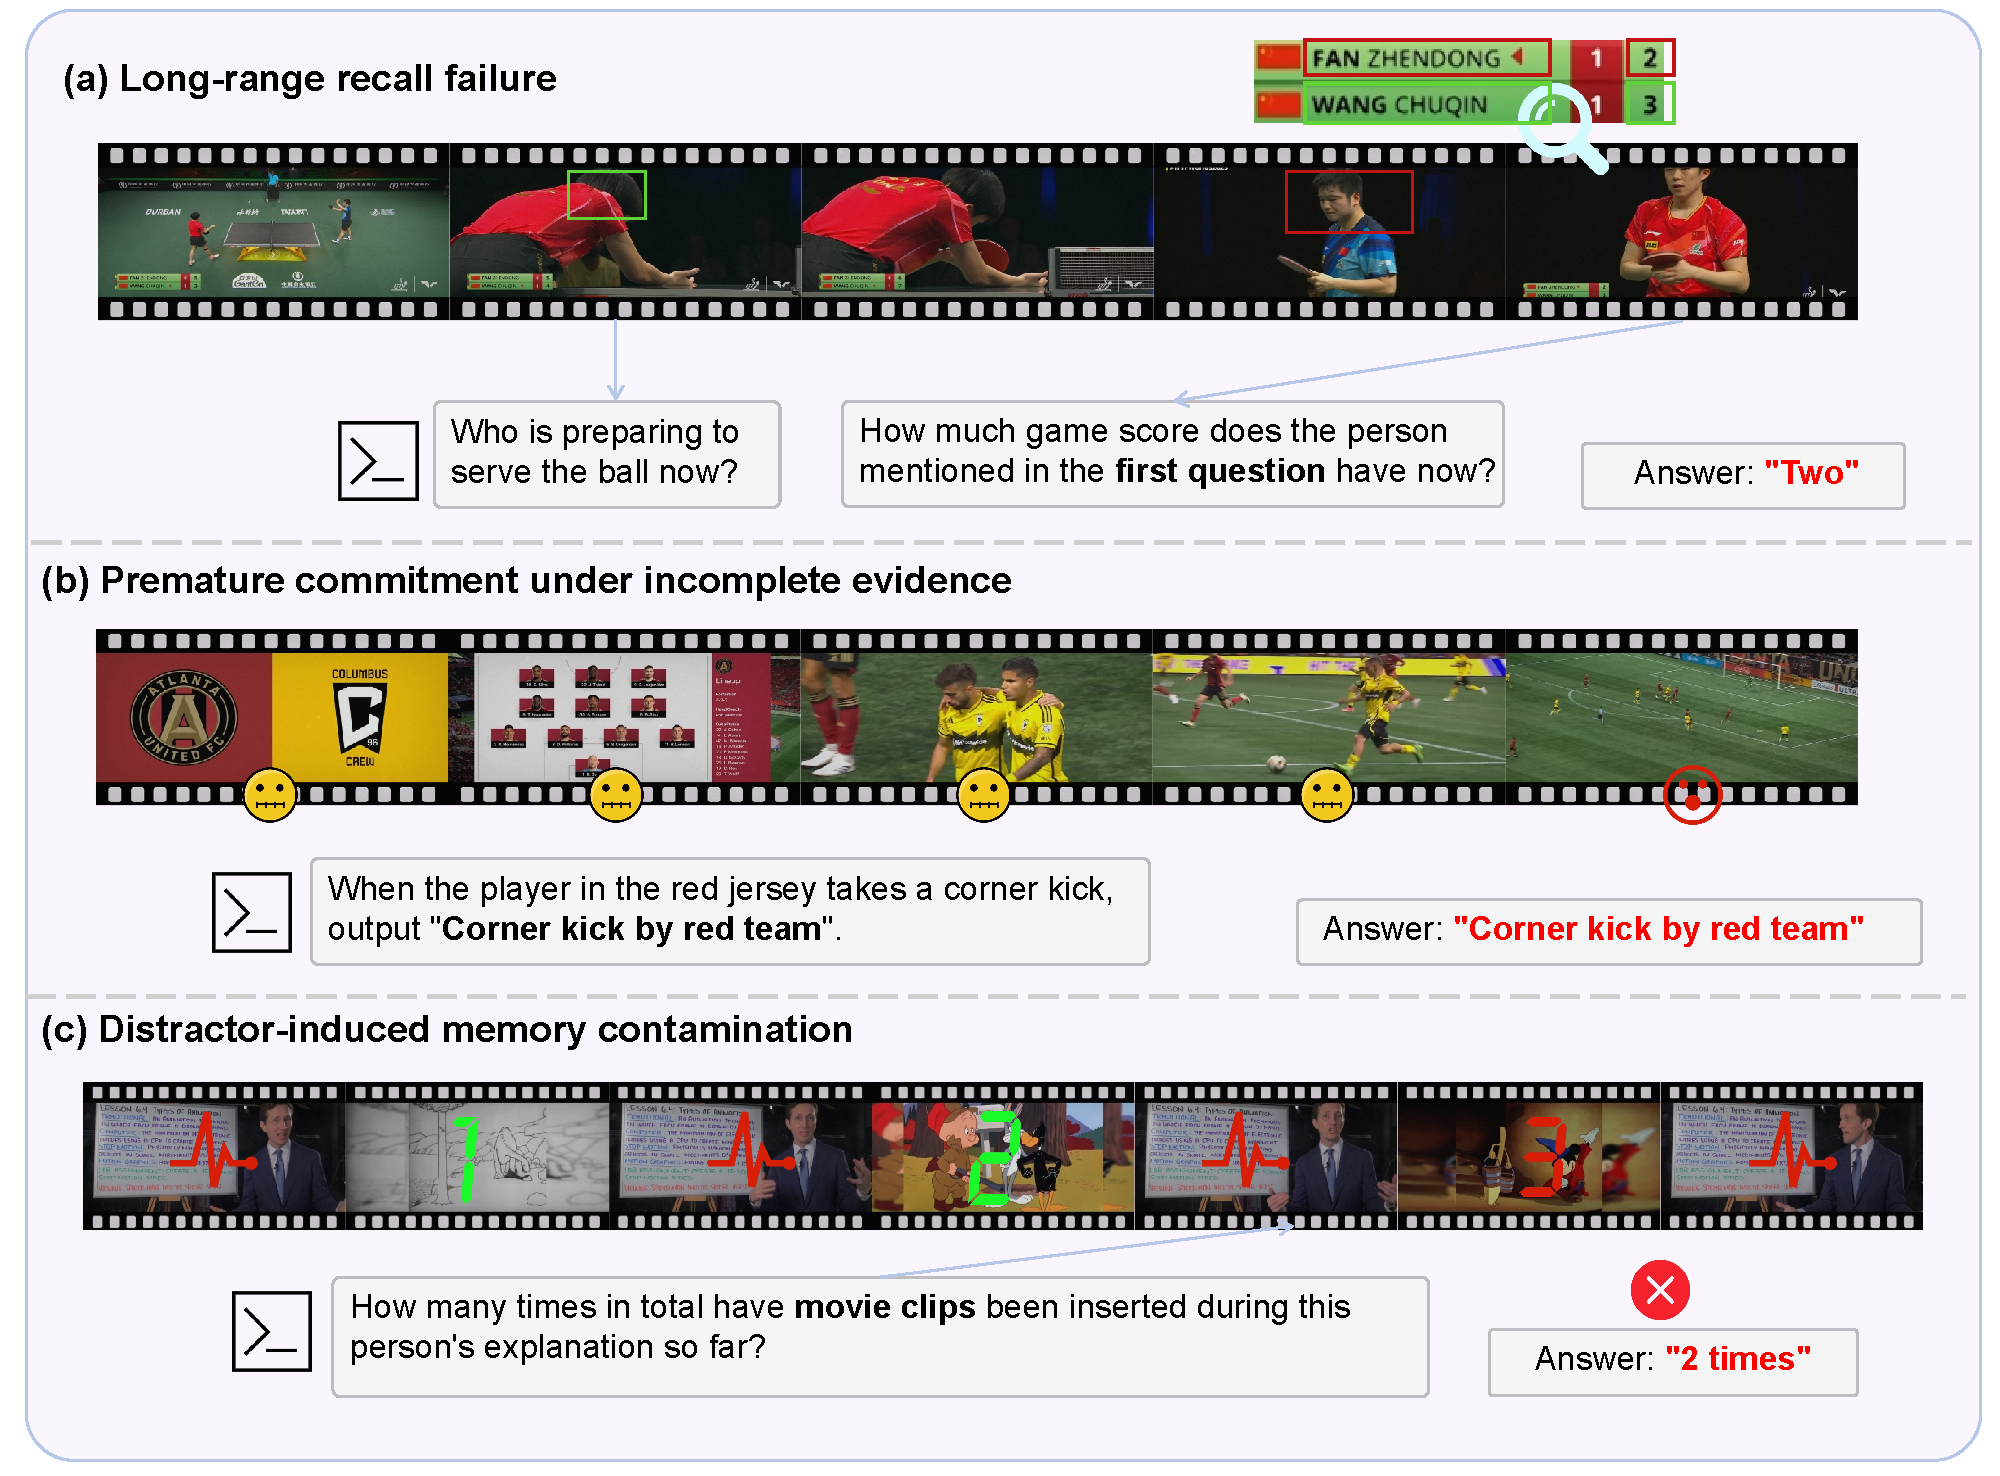
\includegraphics[width=\textwidth,height=0.80\textheight,keepaspectratio]{Figure/Error.pdf}
  \caption{\textbf{Residual failure cases in multi-turn streaming reasoning.}
  \textbf{(a) Long-range recall failure.} The model fails to recover an early fine-grained identity cue across turns. As illustrated in the top row, the \textcolor{green}{green box} marks the correct person referred to in the first question, whereas the \textcolor{red}{red box} marks the person incorrectly retrieved by the model in the later question, indicating that the coarse event context is retained but the specific identity association is lost.
  \textbf{(b) Premature commitment under incomplete evidence.} The middle row shows that, at the queried moment, the decisive visual evidence for whether the red-jersey player is taking a corner kick has not yet become sufficiently clear. Instead of deferring its response until the event is visually confirmed, the model commits to a specific answer too early.
  \textbf{(c) Distractor-induced memory contamination.} The bottom row shows repeated alternation between the speaker and inserted movie clips. Because these inserted clips appear interleaved with the main explanation, the model is distracted by the intervening visual switches and produces an incorrect insertion count.
  These failures are residual edge cases of the three long-horizon behaviors explicitly targeted in Stage~3 training, namely long-term evidence retention, uncertainty handling, and distractor robustness.}
  \label{fig:error_cases}
\end{figure*}

\end{document}
